\documentclass[conference]{IEEEtran}
\IEEEoverridecommandlockouts
\usepackage{cite}
\usepackage{amsmath,amssymb,amsfonts}
\usepackage{graphicx}
\usepackage{booktabs}
\usepackage{textcomp}
\usepackage{xcolor}
\usepackage{tikz}
\usetikzlibrary{positioning,arrows.meta}
\usepackage[hidelinks]{hyperref}
\graphicspath{{./}}

\begin{document}

\title{Feature Reduction, Feature Selection and Metaheuristic Optimisation for Sales-Level Classification on the Noisy Walmart Retail Dataset: A Comparative Analysis}

\author{\IEEEauthorblockN{[Student Name 1]\textsuperscript{1}, [Student Name 2]\textsuperscript{1}}
\IEEEauthorblockA{\textsuperscript{1}\textit{Artificial Intelligence and Data Science Program (AID)} \\
\textit{Egypt-Japan University of Science and Technology (E-JUST)}\\
Alexandria, Egypt \\
\{student1, student2\}@ejust.edu.eg}
}

\maketitle

\begin{abstract}
Weekly department-level retail sales are heavy-tailed, partly missing and influenced by many weak covariates, which makes them a demanding benchmark for feature engineering. We re-formulate the Walmart \emph{Store Sales Forecasting} data (421{,}570 department-weeks, 45 stores, 81 departments) as a balanced three-class \emph{sales-level} problem (Low / Medium / High) and present a comparative analysis of feature reduction, feature selection and classification on it. After a noise audit (64--74\% missing promotions, 8.4\% outliers, negative sales and promotions) and preprocessing into 25 features, we compare ten reduction methods --- PCA, LDA, SVD, Kernel PCA, SNE (implemented from scratch), t-SNE, UMAP, metric and non-metric MDS, Isomap and LLE --- using neighbourhood-classification accuracy, trustworthiness and class silhouette, together with K-Means clustering before and after reduction. We then compare filter, wrapper, embedded and metaheuristic feature selection (Genetic Algorithm, Binary PSO and Simulated Annealing with a size-penalised fitness), and benchmark nine classifiers with an 80/20 hold-out, stratified 5-fold cross-validation, confusion matrices, ROC analysis and learning and validation curves. LightGBM performs best, with 93.44\% test accuracy, macro-F1 0.934 and ROC-AUC 0.991 (5-fold CV 93.42\%$\pm$0.20\%), and only 0.5\% of its errors confuse Low with High. Linear and distance-based classifiers under-fit (44--51\%) because the decisive variable, the department, is a nominal identifier. No unsupervised embedding or clustering recovers the sales levels, but selecting features \emph{before} reduction raises the class information of PCA, t-SNE and UMAP maps by 11--13 points. The GA selects only 6 of 25 features and slightly exceeds the full model (93.70\% accuracy, AUC 0.992) with 42\% less training time, whereas PCA or LDA projections severely degrade the tree ensembles.
\end{abstract}

\begin{IEEEkeywords}
feature selection, dimensionality reduction, genetic algorithm, particle swarm optimisation, simulated annealing, t-SNE, UMAP, LightGBM, retail sales, Walmart
\end{IEEEkeywords}

%========================================================================
\section{Introduction}
%========================================================================
\IEEEPARstart{R}{etail} demand planning is one of the oldest and most economically important applications of data science. A large retailer such as Walmart must decide, every week and for every department of every store, how much stock to order, how many staff hours to schedule, and whether a promotion is worthwhile. The public \emph{Walmart Recruiting -- Store Sales Forecasting} dataset~\cite{kaggle_walmart} captures exactly this setting: 45 stores, 81 departments and almost three years of weekly sales, enriched with weather, fuel price, consumer price index (CPI), unemployment and five anonymised promotional ``MarkDown'' variables.

Most published studies on this dataset frame the task as point regression of weekly sales~\cite{chen2022,akande2022,yao2023,chenwi2024,punati2025}. Point forecasts, however, are notoriously noisy at the department level: sales are heavy-tailed, include negative values (returns), and the promotional variables are missing for most of the history. At the same time, many operational decisions are categorical in nature --- a store manager mainly needs to know whether next week will be a \emph{low}, \emph{medium} or \emph{high} volume week for a department in order to pick a staffing template or a replenishment tier. In this paper we therefore re-formulate the problem as a \textbf{three-class sales-level classification} task, with classes defined by the tertiles of the training distribution.

The reformulation also makes the dataset a demanding, realistic test-bed for the two families of techniques that dominate modern feature engineering: \emph{feature reduction} (projecting the data into a low-dimensional space) and \emph{feature selection} (choosing a subset of the original variables). The data are noisy, mixed-type (identifiers, binary flags, continuous macro-economic indicators) and only weakly structured in Euclidean space, so it is not obvious which techniques help. The contributions of this work are:

\begin{enumerate}
  \item A reproducible preprocessing pipeline and a noise audit of the dataset (Section~\ref{sec:data}), together with a three-class formulation of the sales-level problem.
  \item A side-by-side comparison of \textbf{ten} reduction methods --- three linear (PCA, LDA, SVD) and seven non-linear (Kernel PCA, SNE, t-SNE, UMAP, metric and non-metric MDS, Isomap, LLE) --- measured with three complementary criteria (neighbourhood classification accuracy, trustworthiness and class silhouette), plus a K-Means clustering analysis before and after reduction.
  \item A comparison of \textbf{four} feature-selection families: filter (variance, Spearman, ANOVA-F, $\chi^2$, mutual information with rank fusion), wrapper (sequential forward/backward selection and RFE), embedded (L1, L2, Elastic-Net logistic regression and gradient-boosting gain), and \textbf{metaheuristic} search with a Genetic Algorithm (GA), Binary Particle Swarm Optimisation (BPSO) and Simulated Annealing (SA) using a size-penalised fitness.
  \item A benchmark of nine classifiers under an 80/20 hold-out and stratified 5-fold cross-validation with the full set of metrics (confusion matrix, accuracy, error rate, precision, recall, F-measure, ROC-AUC), an explicit over-/under-fitting diagnosis, and a study of how every selected subset or projection affects the best model.
  \item Evidence that \emph{selection before reduction} --- running the embeddings only on the GA-selected variables --- markedly improves the class structure of the low-dimensional maps.
\end{enumerate}

The remainder of the paper is organised as follows. Section~\ref{sec:related} reviews related work. Section~\ref{sec:data} describes the data and preprocessing. Section~\ref{sec:methods} presents the methods. Section~\ref{sec:results} reports and interprets the results, Section~\ref{sec:compare} compares them with the literature, Section~\ref{sec:discussion} discusses limitations and Section~\ref{sec:conclusion} concludes.

%========================================================================
\section{Related Work}\label{sec:related}
%========================================================================
\subsection{Sales prediction on the Walmart dataset}
Chen~\cite{chen2022} compared multiple linear regression (MLR), Elastic-Net regression (ENR) and polynomial regression on the store-level version of the data and reported $R^2$ values of 0.933 (MLR) and 0.814 (ENR); the polynomial model reached a higher training $R^2$ but a test RMSE many orders of magnitude larger, a textbook case of over-fitting. Akande \emph{et al.}~\cite{akande2022} applied XGBoost to the 45-store data and concluded that gradient boosting is an effective forecaster. Yao~\cite{yao2023} compared decision-tree, random-forest and $k$-nearest-neighbour regressors on the department-level data; the random forest achieved $R^2=0.937$ and MAE $=1937.8$. Chenwi \emph{et al.}~\cite{chenwi2024} benchmarked linear regression, random forest, GBM, XGBoost and LightGBM and found XGBoost best (MAE $=1226.5$), also observing that errors are systematically larger for holiday weeks. More recently, Punati \emph{et al.}~\cite{punati2025} proposed a Temporal Fusion Transformer for multi-horizon probabilistic forecasting, reporting $R^2=0.9875$ and SMAPE $=4.51\%$ against XGBoost, CNN, LSTM and CNN-LSTM baselines.

Two observations motivate the present study. First, all of these works address regression; none studies a categorical sales-level formulation or reports classification metrics. Second, feature engineering in these works is largely manual: none systematically compares reduction methods or selection families, and none uses metaheuristic search over feature subsets.

\subsection{Feature reduction}
Linear reduction includes principal component analysis (PCA)~\cite{pearson1901}, which keeps the directions of maximum variance; linear discriminant analysis (LDA)~\cite{fisher1936}, which is supervised and maximises between-class relative to within-class scatter; and the singular value decomposition (SVD)~\cite{golub1970}, of which truncated SVD is the uncentred analogue of PCA. Non-linear methods either kernelise linear ones --- Kernel PCA~\cite{scholkopf1998} --- or preserve neighbourhood or distance structure. Stochastic Neighbor Embedding (SNE)~\cite{hinton2002} matches Gaussian neighbourhood probabilities in the input and output spaces; t-SNE~\cite{vandermaaten2008} symmetrises them and uses a heavy-tailed Student-$t$ kernel in the output space to alleviate the crowding problem; UMAP~\cite{mcinnes2018} builds a fuzzy topological graph and optimises a cross-entropy layout. Multidimensional scaling preserves pairwise distances either metrically~\cite{torgerson1952} or only through their rank order (non-metric MDS)~\cite{kruskal1964}; Isomap~\cite{tenenbaum2000} replaces Euclidean distances with graph geodesics, and Locally Linear Embedding (LLE)~\cite{roweis2000} preserves local linear reconstruction weights.

\subsection{Feature selection}
Following Guyon and Elisseeff~\cite{guyon2003}, selection methods are grouped into filters, wrappers and embedded methods. Filters score variables independently of any model, for instance by correlation, ANOVA-F, $\chi^2$ or mutual information~\cite{peng2005}. Wrappers~\cite{kohavi1997} search over subsets and score each with a learning algorithm; sequential forward/backward selection and recursive feature elimination (RFE)~\cite{guyon2002} are the classic greedy variants. Embedded methods select during training, e.g.\ through L1 (Lasso)~\cite{tibshirani1996}, L2 (Ridge)~\cite{hoerl1970} or Elastic-Net~\cite{zou2005} penalties, or through tree-ensemble importance. Because subset search is NP-hard, population-based metaheuristics are widely used: Genetic Algorithms~\cite{holland1975,goldberg1989,yang1998}, Binary PSO~\cite{kennedy1997} and Simulated Annealing~\cite{kirkpatrick1983}; Xue \emph{et al.}~\cite{xue2016} survey evolutionary approaches and note that their main weakness is computational cost, which we mitigate here through subsampling, a fast surrogate learner and fitness caching.

%========================================================================
\section{Dataset and Preprocessing}\label{sec:data}
%========================================================================
\subsection{Source data}
The data come from the Kaggle competition \emph{Walmart Recruiting -- Store Sales Forecasting}~\cite{kaggle_walmart} and consist of three related tables. The \texttt{train} table holds 421{,}570 department-week records (\texttt{Store}, \texttt{Dept}, \texttt{Date}, \texttt{Weekly\_Sales}, \texttt{IsHoliday}) for 45 stores and 81 departments, from 5~February~2010 to 26~October~2012. The \texttt{features} table adds, for every store-week, the average regional \texttt{Temperature}, the regional \texttt{Fuel\_Price}, five anonymised promotional variables \texttt{MarkDown1}--\texttt{MarkDown5}, the \texttt{CPI} and the regional \texttt{Unemployment} rate. The \texttt{stores} table gives each store's \texttt{Type} (A, B or C) and floor \texttt{Size}. The three tables are joined on (\texttt{Store}, \texttt{Date}) and \texttt{Store}, respectively. The four holiday weeks flagged by Walmart --- Super Bowl, Labor Day, Thanksgiving and Christmas --- are known to be weighted five times more heavily in the original competition metric.

\subsection{Noise audit}
The cover specification of this project asks for a ``difficult dataset with noise''. Table~\ref{tab:noise} quantifies why the Walmart data qualify. The target is extremely right-skewed (skewness 3.26; mean \$15{,}981 versus median \$7{,}612; maximum \$693{,}099). 1{,}285 records have \emph{negative} sales (net returns), and 35{,}521 records (8.4\%) lie outside the $1.5\times$IQR whiskers. The promotional variables are missing for 64--74\% of the rows, mostly because MarkDowns were only recorded from November 2011 onward, and 1{,}568 MarkDown values are negative, which is impossible for a discount amount and must be treated as entry errors. Finally, the store-week context variables (temperature, fuel price, CPI, unemployment) are measured at the store or region level and are therefore identical for all $\approx$74 departments of a store in a given week: for the department-level target they act as weak, highly redundant covariates.

\begin{table}[!t]
\caption{Noise and quality issues in the merged dataset (421{,}570 rows)}
\label{tab:noise}
\centering
\begin{tabular}{lrr}
\toprule
Issue & Count & \% rows \\
\midrule
Negative weekly sales (returns) & 1{,}285 & 0.30 \\
Weekly-sales outliers ($1.5\times$IQR) & 35{,}521 & 8.43 \\
MarkDown1 missing & 270{,}889 & 64.26 \\
MarkDown2 missing & 310{,}322 & 73.61 \\
MarkDown3 missing & 284{,}479 & 67.48 \\
MarkDown4 missing & 286{,}603 & 67.98 \\
MarkDown5 missing & 270{,}138 & 64.08 \\
Negative MarkDown values & 1{,}568 & 0.37 \\
Holiday-week rows & 29{,}661 & 7.04 \\
Skewness of \texttt{Weekly\_Sales} & \multicolumn{2}{c}{3.26} \\
\bottomrule
\end{tabular}
\end{table}

\subsection{Target definition}
We define three ordered classes by the 33.3th and 66.7th percentiles of \texttt{Weekly\_Sales}: \textbf{Low} ($\le\$3{,}521.78$), \textbf{Medium} ($\$3{,}521.78$--$\$14{,}599.76$) and \textbf{High} ($>\$14{,}599.76$). By construction the classes are balanced (140{,}524 / 140{,}523 / 140{,}523 rows), so accuracy is a meaningful headline metric and the chance level is 33.3\%. Negative sales are kept --- they are genuine business events --- and fall into the Low class.

\subsection{Preprocessing}
\begin{enumerate}
\item \textbf{Missing promotions.} A missing MarkDown means that no promotion was recorded, so it is replaced by zero, and a binary \texttt{MarkDown\_Available} flag preserves the information that the value was missing.
\item \textbf{Promotion noise.} Negative MarkDowns are clipped to zero, and each MarkDown is winsorised at its 99.5th percentile to limit the leverage of extreme promotions.
\item \textbf{Calendar features.} From \texttt{Date} we derive \texttt{Year}, \texttt{Month}, ISO \texttt{Week} and \texttt{Day}; the signed number of days to Thanksgiving and to Christmas of the same year; and binary Super Bowl and Labor Day indicators.
\item \textbf{Encoding.} Store \texttt{Type} is one-hot encoded (\texttt{Type\_A}, \texttt{Type\_B}, \texttt{Type\_C}) and \texttt{IsHoliday} is cast to an integer.
\end{enumerate}
The final design matrix has \textbf{25 features}, listed in Table~\ref{tab:features}, and no missing values.

\begin{table}[!t]
\caption{The 25 model features}
\label{tab:features}
\centering
\begin{tabular}{p{1.9cm}p{5.9cm}}
\toprule
Group & Features \\
\midrule
Identity & Store, Dept \\
Store & Size, Type\_A, Type\_B, Type\_C \\
Economy & Temperature, Fuel\_Price, CPI, Unemployment \\
Promotion & MarkDown1--5, MarkDown\_Available \\
Calendar & IsHoliday, Year, Month, Week, Day, Days\_to\_Thanksgiving, Days\_to\_Christmas, SuperBowl, LaborDay \\
\bottomrule
\end{tabular}
\end{table}

\subsection{Exploratory analysis}
Fig.~\ref{fig:eda} summarises the data before any reduction. Total chain-wide sales are flat for most of the year and spike sharply in the flagged Thanksgiving week (about \$66M versus a typical \$45--50M) and in the week \emph{before} Christmas (up to \$81M). The flagged Christmas week itself, which ends on the last Friday of December, is actually a dip, and the Super Bowl and Labor Day weeks show no visible spike. Only one of the four official holiday weeks therefore coincides with a peak, which already hints that the \texttt{IsHoliday} flag is a weak predictor. Store size increases from Type C to Type A stores; within Types A and B the High class is associated with larger stores, whereas Type C stores all have almost the same size. Fig.~\ref{fig:corr} shows the Spearman correlation matrix: the strongest monotone association with the sales class is \texttt{Size} ($\rho=0.26$), followed by the store-type dummies ($|\rho|=0.10$--$0.19$); all other features have $|\rho|<0.08$. In particular, \texttt{Dept} has an almost zero rank correlation with the class ($\rho=-0.03$) even though, as shown later, it is by far the most informative variable: its effect is strong but entirely \emph{non-monotone}, because department numbers are arbitrary identifiers. The calendar variables \texttt{Week}, \texttt{Month}, \texttt{Days\_to\_Thanksgiving} and \texttt{Days\_to\_Christmas} are almost perfectly collinear, and so are the five MarkDowns, which indicates substantial redundancy for the reduction and selection methods to exploit.

\begin{figure*}[!t]
\centering
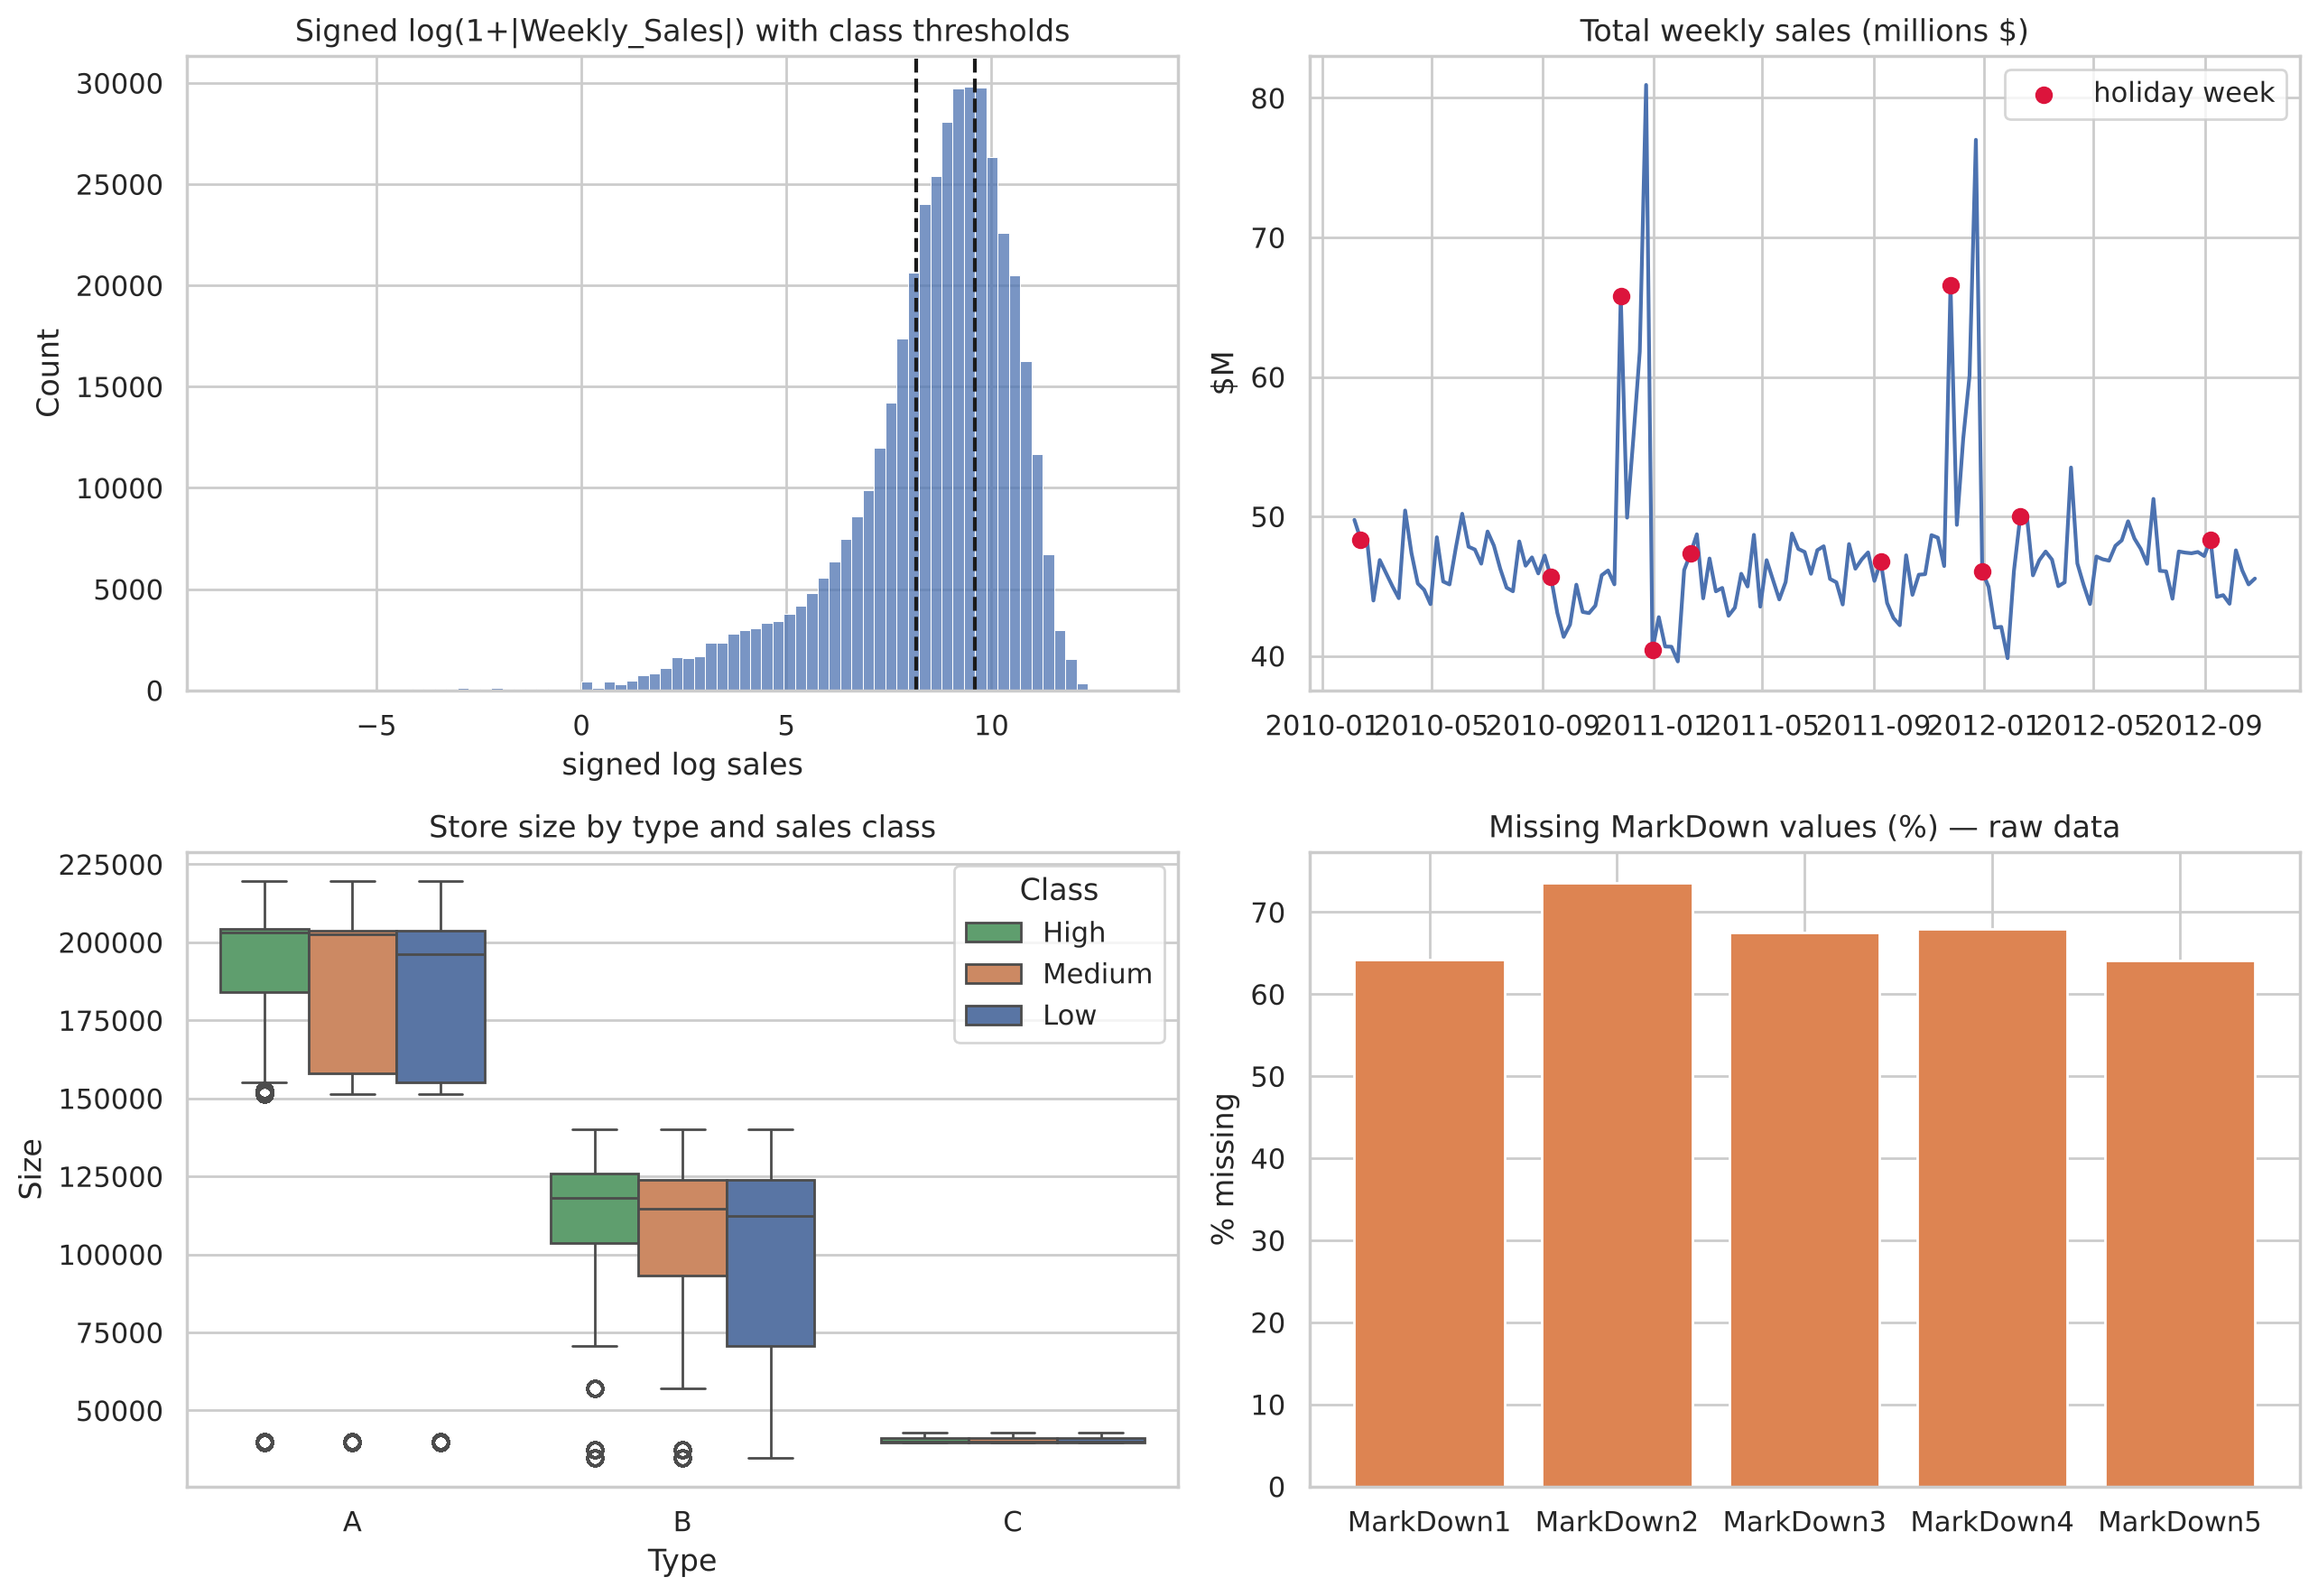
\includegraphics[width=0.86\textwidth]{figures/01_eda_overview.png}
\caption{Exploratory analysis before reduction. Top-left: signed $\log(1+|\text{sales}|)$ with the two class thresholds (dashed). Top-right: chain-wide weekly sales with holiday weeks in red. Bottom-left: store size by type and class. Bottom-right: share of missing MarkDown values in the raw data.}
\label{fig:eda}
\end{figure*}

\begin{figure}[!t]
\centering
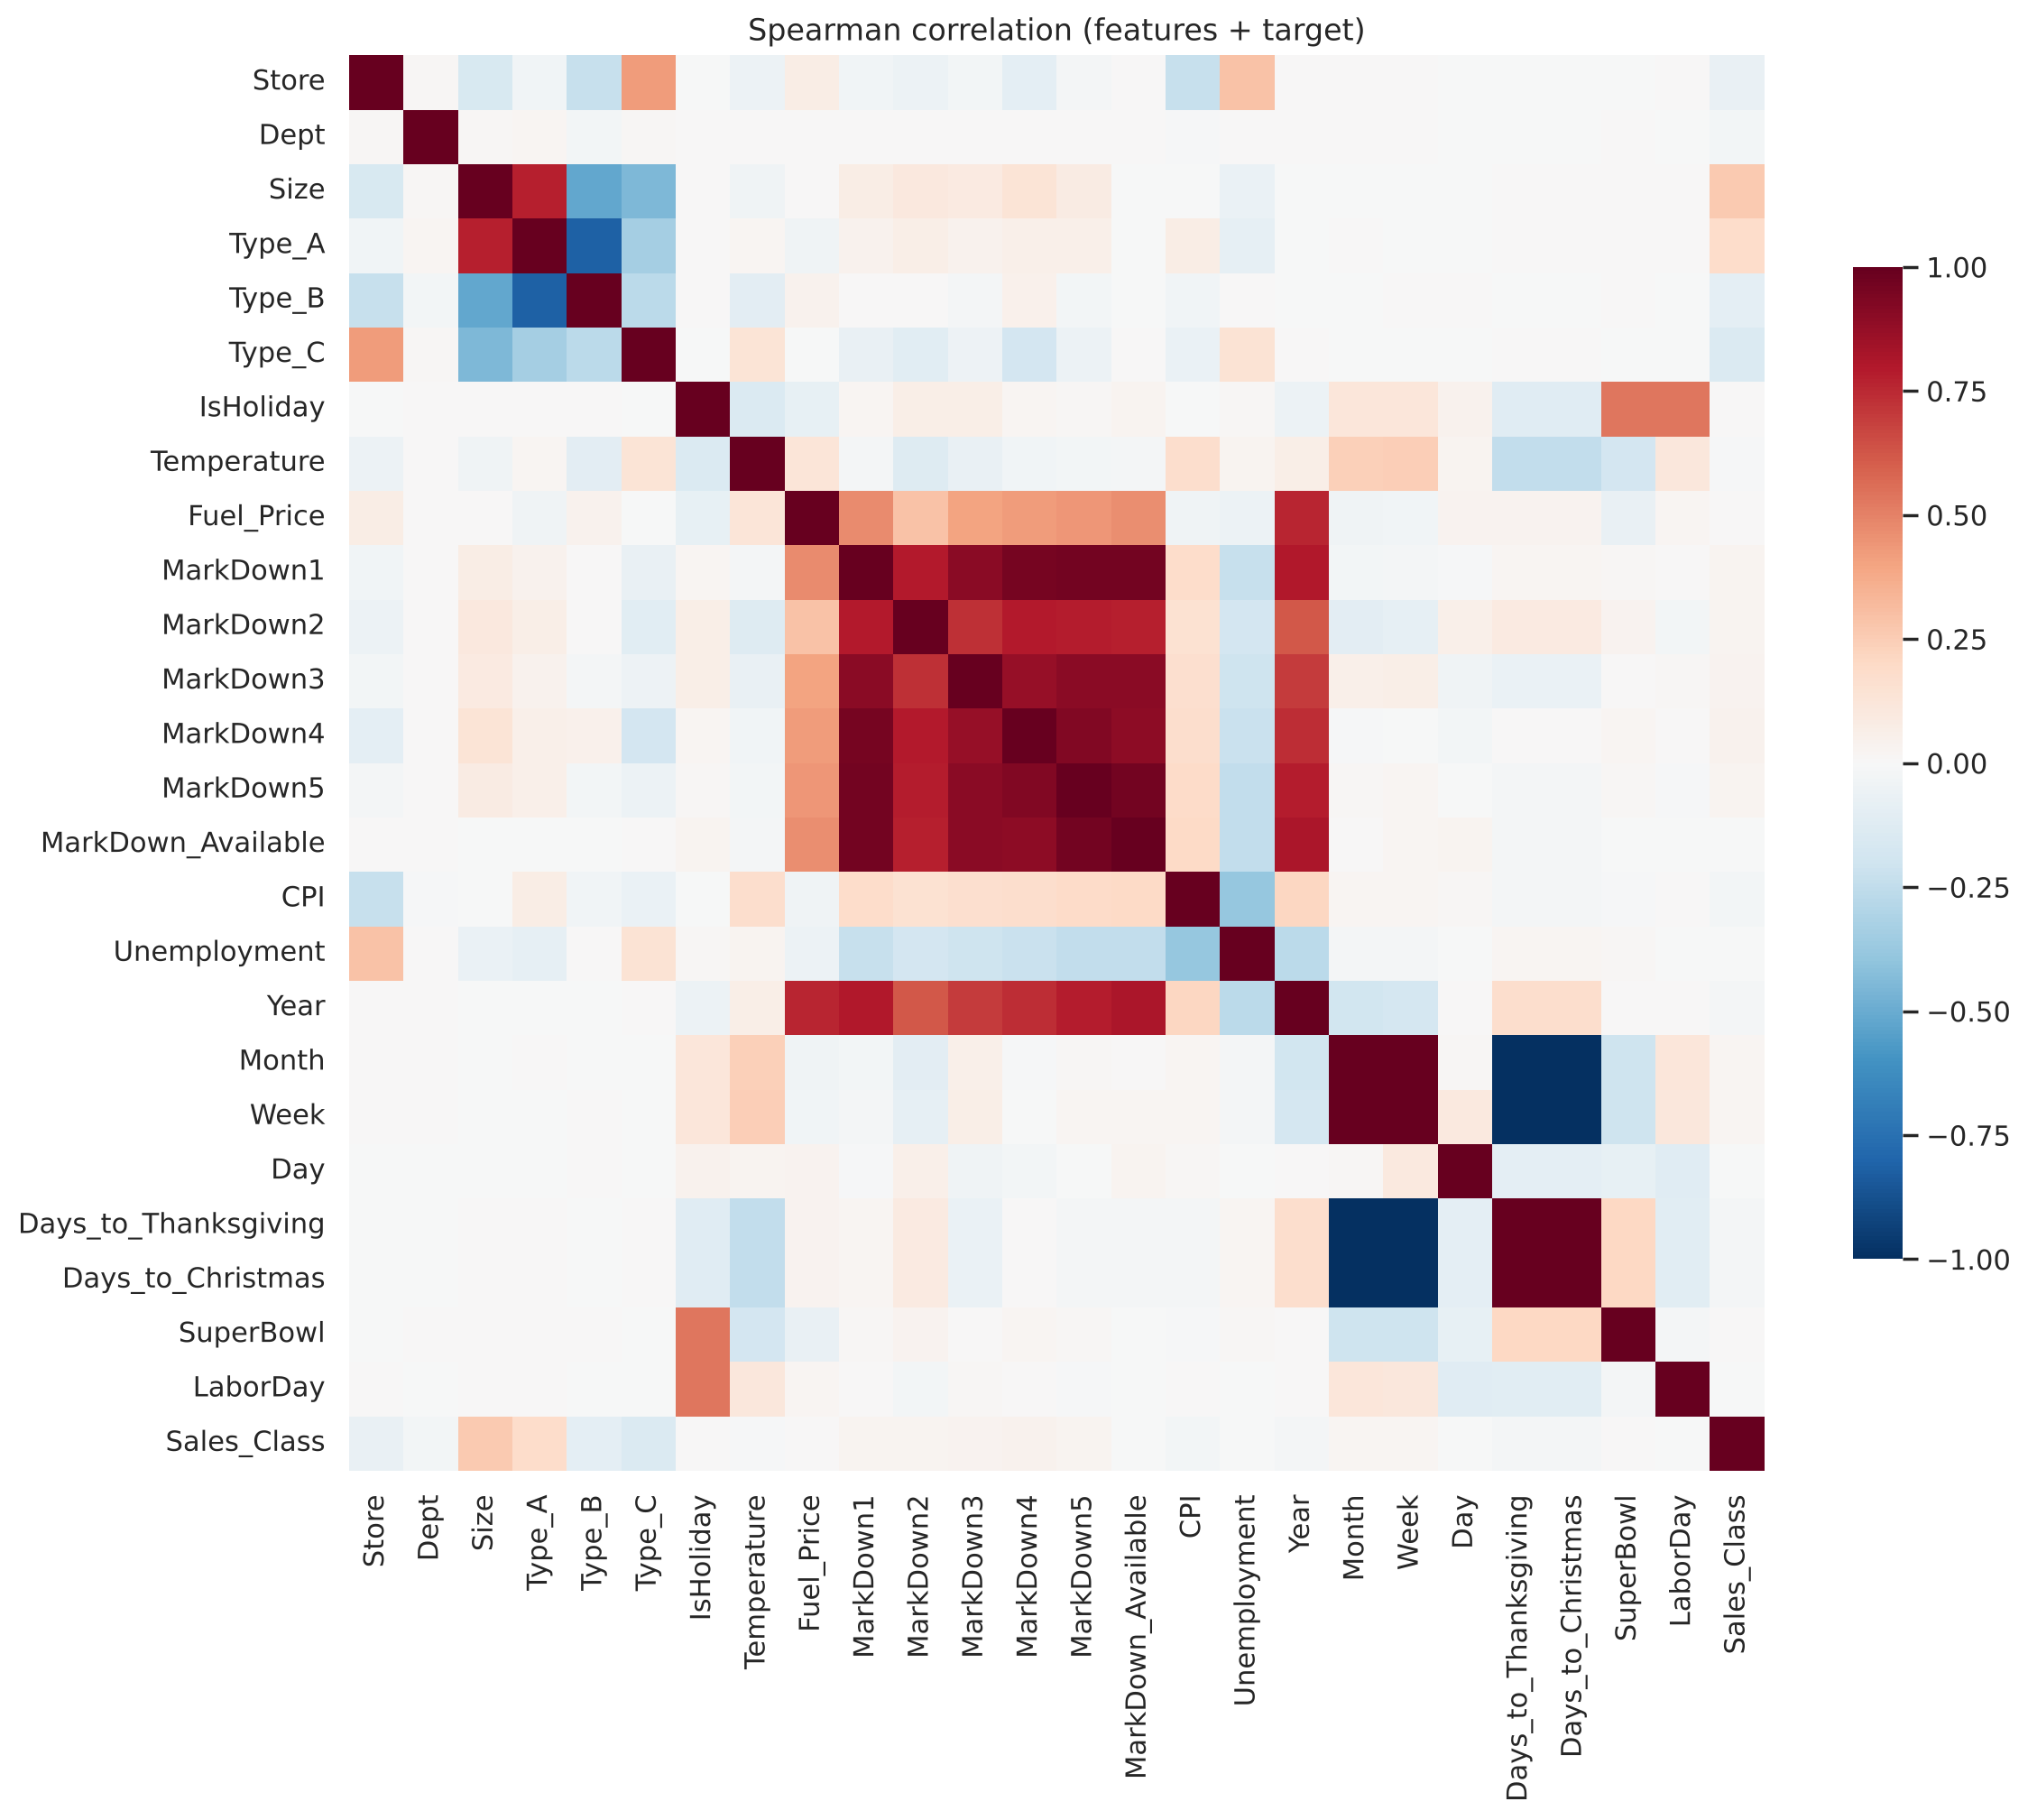
\includegraphics[width=\columnwidth]{figures/02_correlation.png}
\caption{Spearman correlation between the 25 features and the ordinal sales class (last row/column).}
\label{fig:corr}
\end{figure}

\subsection{Sampling and splitting}
Training nine models with 5-fold cross-validation, and running three metaheuristics that each evaluate several hundred feature subsets, on 421{,}570 rows is beyond the two-core, 8-GB machine used for this study. We therefore draw a \textbf{stratified sample of 100{,}000 rows} (23.7\% of the data) and split it \textbf{80/20} with stratification into 80{,}000 training and 20{,}000 test rows. Feature selection uses a 20{,}000-row subsample of the training split only, so the test rows never influence which features are chosen. The manifold methods, whose cost grows quadratically or cubically with $n$, use a 3{,}000-point subsample of the training split (1{,}500 points for SNE and 1{,}000 for MDS).


%========================================================================
\section{Methodology}\label{sec:methods}
%========================================================================
Fig.~\ref{fig:pipeline} summarises the experimental pipeline. All randomness is controlled with a single seed (42) and all experiments were run with scikit-learn~\cite{pedregosa2011}, LightGBM~\cite{ke2017}, XGBoost~\cite{chen2016xgb} and umap-learn~\cite{mcinnes2018}. The complete code is available in the accompanying Jupyter notebook.

\begin{figure}[!t]
\centering
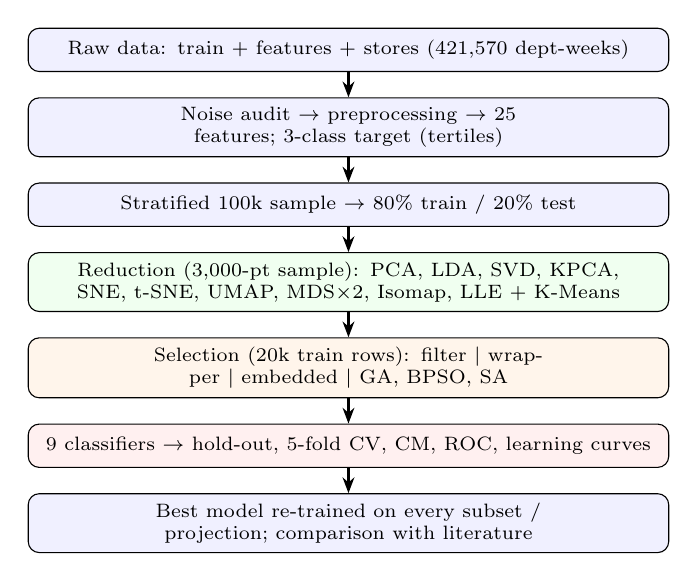
\begin{tikzpicture}[node distance=0.32cm, every node/.style={font=\scriptsize},
  box/.style={draw, rounded corners, fill=blue!6, text width=7.9cm, minimum height=0.55cm, align=center},
  arr/.style={-{Stealth[length=2mm]}, thick}]
\node[box] (a) {Raw data: train + features + stores (421{,}570 dept-weeks)};
\node[box, below=of a] (b) {Noise audit $\rightarrow$ preprocessing $\rightarrow$ 25 features; 3-class target (tertiles)};
\node[box, below=of b] (c) {Stratified 100k sample $\rightarrow$ 80\% train / 20\% test};
\node[box, below=of c, fill=green!6] (d) {Reduction (3{,}000-pt sample): PCA, LDA, SVD, KPCA, SNE, t-SNE, UMAP, MDS$\times$2, Isomap, LLE + K-Means};
\node[box, below=of d, fill=orange!8] (e) {Selection (20k train rows): filter $|$ wrapper $|$ embedded $|$ GA, BPSO, SA};
\node[box, below=of e, fill=red!6] (f) {9 classifiers $\rightarrow$ hold-out, 5-fold CV, CM, ROC, learning curves};
\node[box, below=of f] (g) {Best model re-trained on every subset / projection; comparison with literature};
\foreach \u/\v in {a/b,b/c,c/d,d/e,e/f,f/g} \draw[arr] (\u) -- (\v);
\end{tikzpicture}
\caption{Experimental pipeline. Feature selection only ever sees training rows; the 20\% test split is touched once per model.}
\label{fig:pipeline}
\end{figure}

\subsection{Linear reduction}
Let $\mathbf{X}\in\mathbb{R}^{n\times d}$ be the standardised data matrix. \textbf{PCA} computes the eigen-decomposition of the covariance $\mathbf{C}=\frac{1}{n-1}\mathbf{X}^\top\mathbf{X}=\mathbf{V}\boldsymbol{\Lambda}\mathbf{V}^\top$ and projects onto the $k$ leading eigenvectors, $\mathbf{Z}=\mathbf{X}\mathbf{V}_k$; the explained-variance ratio of component $j$ is $\lambda_j/\sum_i\lambda_i$. \textbf{LDA} solves the generalised eigenproblem $\mathbf{S}_B\mathbf{w}=\lambda\mathbf{S}_W\mathbf{w}$ with between-class scatter $\mathbf{S}_B=\sum_c n_c(\boldsymbol{\mu}_c-\boldsymbol{\mu})(\boldsymbol{\mu}_c-\boldsymbol{\mu})^\top$ and within-class scatter $\mathbf{S}_W=\sum_c\sum_{i\in c}(\mathbf{x}_i-\boldsymbol{\mu}_c)(\mathbf{x}_i-\boldsymbol{\mu}_c)^\top$; with $C=3$ classes it yields at most $C-1=2$ discriminant axes. \textbf{Truncated SVD} factorises $\mathbf{X}\approx\mathbf{U}_k\boldsymbol{\Sigma}_k\mathbf{V}_k^\top$ and keeps $\mathbf{Z}=\mathbf{U}_k\boldsymbol{\Sigma}_k$; on centred data it coincides with PCA, which serves as a sanity check.

\subsection{Non-linear reduction}
\textbf{Kernel PCA} performs PCA in a feature space induced by the RBF kernel $k(\mathbf{x},\mathbf{x}')=\exp(-\gamma\|\mathbf{x}-\mathbf{x}'\|^2)$ by eigen-decomposing the centred Gram matrix; $\gamma$ was chosen from $\{0.005,0.02,0.05,0.1\}$ by kNN accuracy. \textbf{SNE} defines conditional probabilities
\begin{equation}
p_{j|i}=\frac{\exp(-\|\mathbf{x}_i-\mathbf{x}_j\|^2/2\sigma_i^2)}{\sum_{k\neq i}\exp(-\|\mathbf{x}_i-\mathbf{x}_k\|^2/2\sigma_i^2)},
\end{equation}
with $\sigma_i$ found by binary search so that the perplexity $2^{H(P_i)}$ equals 30, analogous Gaussian $q_{j|i}$ in the 2-D space, and minimises $\sum_i \mathrm{KL}(P_i\|Q_i)$ whose gradient is
\begin{equation}
\frac{\partial C}{\partial\mathbf{y}_i}=2\sum_j\left(p_{j|i}-q_{j|i}+p_{i|j}-q_{i|j}\right)(\mathbf{y}_i-\mathbf{y}_j).
\end{equation}
Because scikit-learn does not provide SNE, we implemented it from scratch (gradient descent with momentum 0.5$\to$0.8, learning rate 0.1, 600 iterations, gradient clipping to protect against ``hub'' points). \textbf{t-SNE} uses symmetric joint probabilities and the Student-$t$ output kernel $q_{ij}\propto(1+\|\mathbf{y}_i-\mathbf{y}_j\|^2)^{-1}$ (perplexity 30, PCA initialisation). \textbf{UMAP} uses 15 neighbours and a minimum distance of 0.1. \textbf{Metric MDS} minimises the raw stress $\sum_{i<j}(\|\mathbf{y}_i-\mathbf{y}_j\|-\delta_{ij})^2$ with the SMACOF algorithm; \textbf{non-metric MDS} replaces $\delta_{ij}$ by a monotone (isotonic) transformation of it. \textbf{Isomap} (10 neighbours) applies classical MDS to shortest-path distances on the $k$NN graph, and \textbf{LLE} (12 neighbours) finds weights $\mathbf{W}$ minimising $\sum_i\|\mathbf{x}_i-\sum_j W_{ij}\mathbf{x}_j\|^2$ and then low-dimensional points preserving the same weights.

\subsection{Embedding quality criteria}
Because a 2-D picture can be misleading, every embedding is scored with three numbers: (i) the 5-fold accuracy of a 5-NN classifier trained \emph{in} the embedding, which measures how much class information survives; (ii) trustworthiness~\cite{venna2006},
\begin{equation}
T(k)=1-\frac{2}{nk(2n-3k-1)}\sum_{i=1}^{n}\sum_{j\in U_i^{(k)}}\left(r(i,j)-k\right),
\end{equation}
where $U_i^{(k)}$ are points that are among the $k=10$ nearest neighbours of $i$ in the embedding but not in the input space and $r(i,j)$ is their rank in the input space; and (iii) the silhouette~\cite{rousseeuw1987} of the true classes. For clustering we run K-Means~\cite{lloyd1982} with $k=3$ and report the silhouette of the found clusters together with the Adjusted Rand Index (ARI)~\cite{hubert1985} and normalised mutual information (NMI) against the true sales classes.

\subsection{Feature selection}
All selectors operate on a 20{,}000-row subsample of the \emph{training} split; subset sizes for ranked or greedy methods are fixed at $K=10$ of 25 features.

\textbf{Filter.} For every feature we compute the variance after min--max scaling, the absolute Spearman correlation with the ordinal class, the ANOVA $F$ statistic, the $\chi^2$ statistic on min--max scaled values and the mutual information (with discrete treatment for variables having fewer than 60 distinct values). The four relevance scores are converted to ranks and averaged (\emph{rank fusion}); the ten best-ranked features form the filter subset.

\textbf{Wrapper.} Sequential forward selection (SFS) starts from the empty set and greedily adds the feature that most improves the 3-fold macro-F1 of a fast LightGBM (60 trees); sequential backward selection starts from all features and removes greedily. RFE repeatedly fits a 60-tree random forest and drops the least important feature.

\textbf{Embedded.} Multinomial logistic regression with $C=0.05$ is trained on standardised data under three penalties,
\begin{equation}
\Omega(\mathbf{W})=\alpha\|\mathbf{W}\|_1+\tfrac{1-\alpha}{2}\|\mathbf{W}\|_2^2,\quad \alpha\in\{1,\,0,\,0.5\},
\end{equation}
i.e.\ L1 (Lasso), L2 (Ridge) and Elastic-Net. A feature is kept by L1/Elastic-Net if the norm of its coefficient vector across the three classes is non-zero; for L2, which never produces exact zeros, the ten largest norms are kept. LightGBM total-gain importance is reported as a tree-based embedded reference.

\textbf{Metaheuristics.} A candidate solution is a bit-mask $\mathbf{b}\in\{0,1\}^{25}$. All three searches maximise the same fitness
\begin{equation}
f(\mathbf{b})=\overline{F_1}^{\,3\text{-fold}}(\mathbf{b})-\lambda\frac{\|\mathbf{b}\|_1}{25},\qquad \lambda=0.02,
\label{eq:fitness}
\end{equation}
which trades predictive quality against subset size; evaluated masks are cached so that repeated individuals cost nothing. The \textbf{GA} uses a population of 24, 20 generations, tournament selection ($k=3$), uniform crossover ($p_c=0.9$), bit-flip mutation ($p_m=1/25$) and elitism of two. \textbf{BPSO} uses 20 particles and 20 iterations with inertia $w=0.7$, $c_1=c_2=1.5$, velocity clamp $\pm4$ and the sigmoid transfer $P(b_{id}=1)=1/(1+e^{-v_{id}})$. \textbf{SA} performs 300 single-bit-flip moves with initial temperature $T_0=0.02$, geometric cooling $\alpha=0.985$ and the Metropolis acceptance rule $P=\exp(\Delta f/T)$.

\subsection{Classifiers}
Nine classifiers cover linear, probabilistic, instance-based, single-tree, bagging, boosting and neural families: logistic regression; Gaussian naive Bayes; $k$-NN ($k=15$); an unpruned decision tree; random forest~\cite{breiman2001} (150 trees, minimum leaf size 2); extra trees~\cite{geurts2006} (150 trees, minimum leaf size 2); a multilayer perceptron (128--64 ReLU units, early stopping); XGBoost~\cite{chen2016xgb} (400 trees, depth 8, learning rate 0.1, row/column subsampling 0.9); and LightGBM~\cite{ke2017} (500 trees, 127 leaves, learning rate 0.05). Scale-sensitive models are wrapped in a standardisation pipeline fitted on the training fold only.

\subsection{Evaluation protocol}
From the 421{,}570 rows we draw a stratified sample of 100{,}000 and split it 80/20 with stratification. On the 20\% test set we report the confusion matrix and
\begin{align}
\text{Accuracy}&=\tfrac{\sum_c TP_c}{N},\qquad \text{Error rate}=1-\text{Accuracy},\\
\text{Precision}&=\tfrac{1}{C}\sum_c\tfrac{TP_c}{TP_c+FP_c},\quad \text{Recall}=\tfrac{1}{C}\sum_c\tfrac{TP_c}{TP_c+FN_c},\\
F_1&=\tfrac{1}{C}\sum_c\tfrac{2P_cR_c}{P_c+R_c},
\end{align}
(macro averages) and the one-vs-rest macro ROC-AUC~\cite{fawcett2006}. Stratified 5-fold cross-validation~\cite{kohavi1995} on the full 100k sample gives the mean and standard deviation of accuracy, macro-F1 and AUC. A model is labelled \emph{over-fitting} when its train--test accuracy gap exceeds 5 percentage points, and \emph{under-fitting} when its test accuracy is below 70\% with a small gap. Learning curves of the best model and a validation curve of the decision-tree depth make the bias--variance behaviour visible.

%========================================================================
\section{Results and Interpretation}\label{sec:results}
%========================================================================

\subsection{Linear feature reduction}
\textbf{PCA.} On the standardised 80{,}000-row training matrix the first two principal components explain 17.5\% and 14.9\% of the variance, and \textbf{16 of the 25 components} are needed to reach 95\% (Fig.~\ref{fig:pca}). This flat spectrum is typical of noisy, weakly correlated data. The last four components carry essentially zero variance because \texttt{Type\_A}+\texttt{Type\_B}+\texttt{Type\_C}$=1$ and because \texttt{Week}, \texttt{Days\_to\_Thanksgiving} and \texttt{Days\_to\_Christmas} are exact linear functions of each other within a year, which confirms the redundancy noted in Section~\ref{sec:data}. The loadings are easy to interpret: PC1 is a \emph{seasonality} axis (equal loadings of 0.43 on \texttt{Week}, \texttt{Month} and the two days-to-holiday variables), and PC2 is a \emph{promotion-era} axis (\texttt{MarkDown\_Available} 0.41, \texttt{MarkDown5} 0.37, \texttt{MarkDown1} 0.36, \texttt{Year} 0.34). Neither axis involves \texttt{Dept} or \texttt{Size}, the two most predictive features, so the variance-maximising view of the data is largely orthogonal to the sales-level question. In Fig.~\ref{fig:linear} the PCA projection therefore shows clear structure --- parallel bands along the seasonal and promotion-era axes --- but the three classes are completely mixed.

\textbf{LDA.} Because it uses the labels, LDA is the only linear method that targets class separation. The first discriminant explains 84.3\% of the between-class variance. In the 2-D LDA map a Low-dominated region and a High-dominated region become visible, and the 5-NN accuracy in the embedding is the best of all ten 2-D maps (46.3\%; Table~\ref{tab:emb}). Used directly as a linear classifier, however, LDA reaches only 44.1\% test accuracy. The class boundaries are therefore not linear in the original features, which foreshadows the poor results of the linear classifiers in Section~\ref{sec:res:models}.

\textbf{SVD.} Truncated SVD on standardised (hence centred) data reproduces the PCA solution up to sign: the explained-variance ratios of the first two components (17.4\% and 15.0\%), the 5-NN accuracy (37.1\%) and the trustworthiness (0.889) are identical to PCA's within rounding. The leading singular values are 591.7, 545.4, 447.6, 392.6 and 375.9. This sanity check confirms the equivalence $\mathbf{X}=\mathbf{U}\boldsymbol{\Sigma}\mathbf{V}^\top\Rightarrow\mathbf{C}=\mathbf{V}\frac{\boldsymbol{\Sigma}^2}{n-1}\mathbf{V}^\top$ for centred $\mathbf{X}$.

\begin{figure*}[!t]
\centering
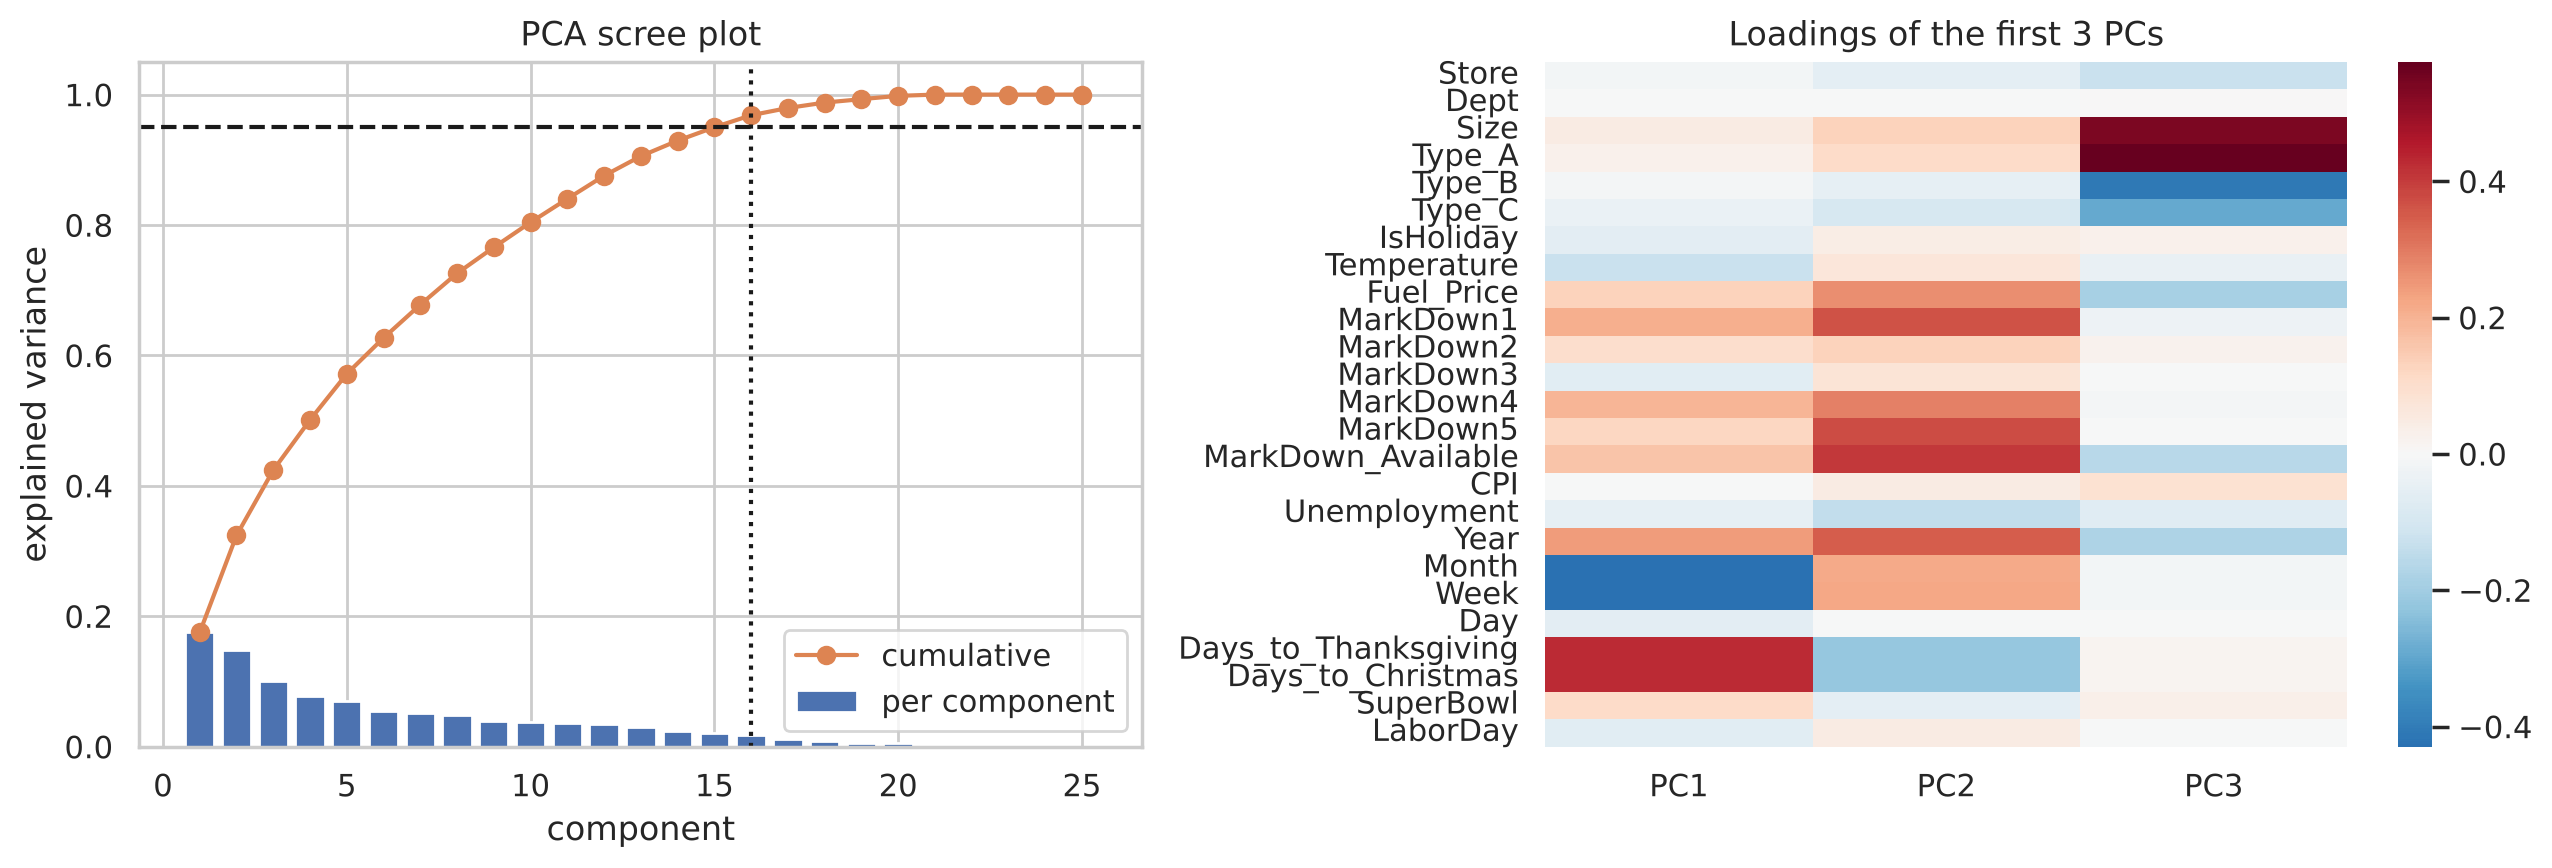
\includegraphics[width=0.85\textwidth]{figures/04_pca_scree_loadings.png}
\caption{PCA on the training split. Left: scree plot with the cumulative explained variance (16 components reach 95\%). Right: loadings of the first three components --- PC1 is seasonality, PC2 is the promotion era.}
\label{fig:pca}
\end{figure*}

\begin{figure*}[!t]
\centering
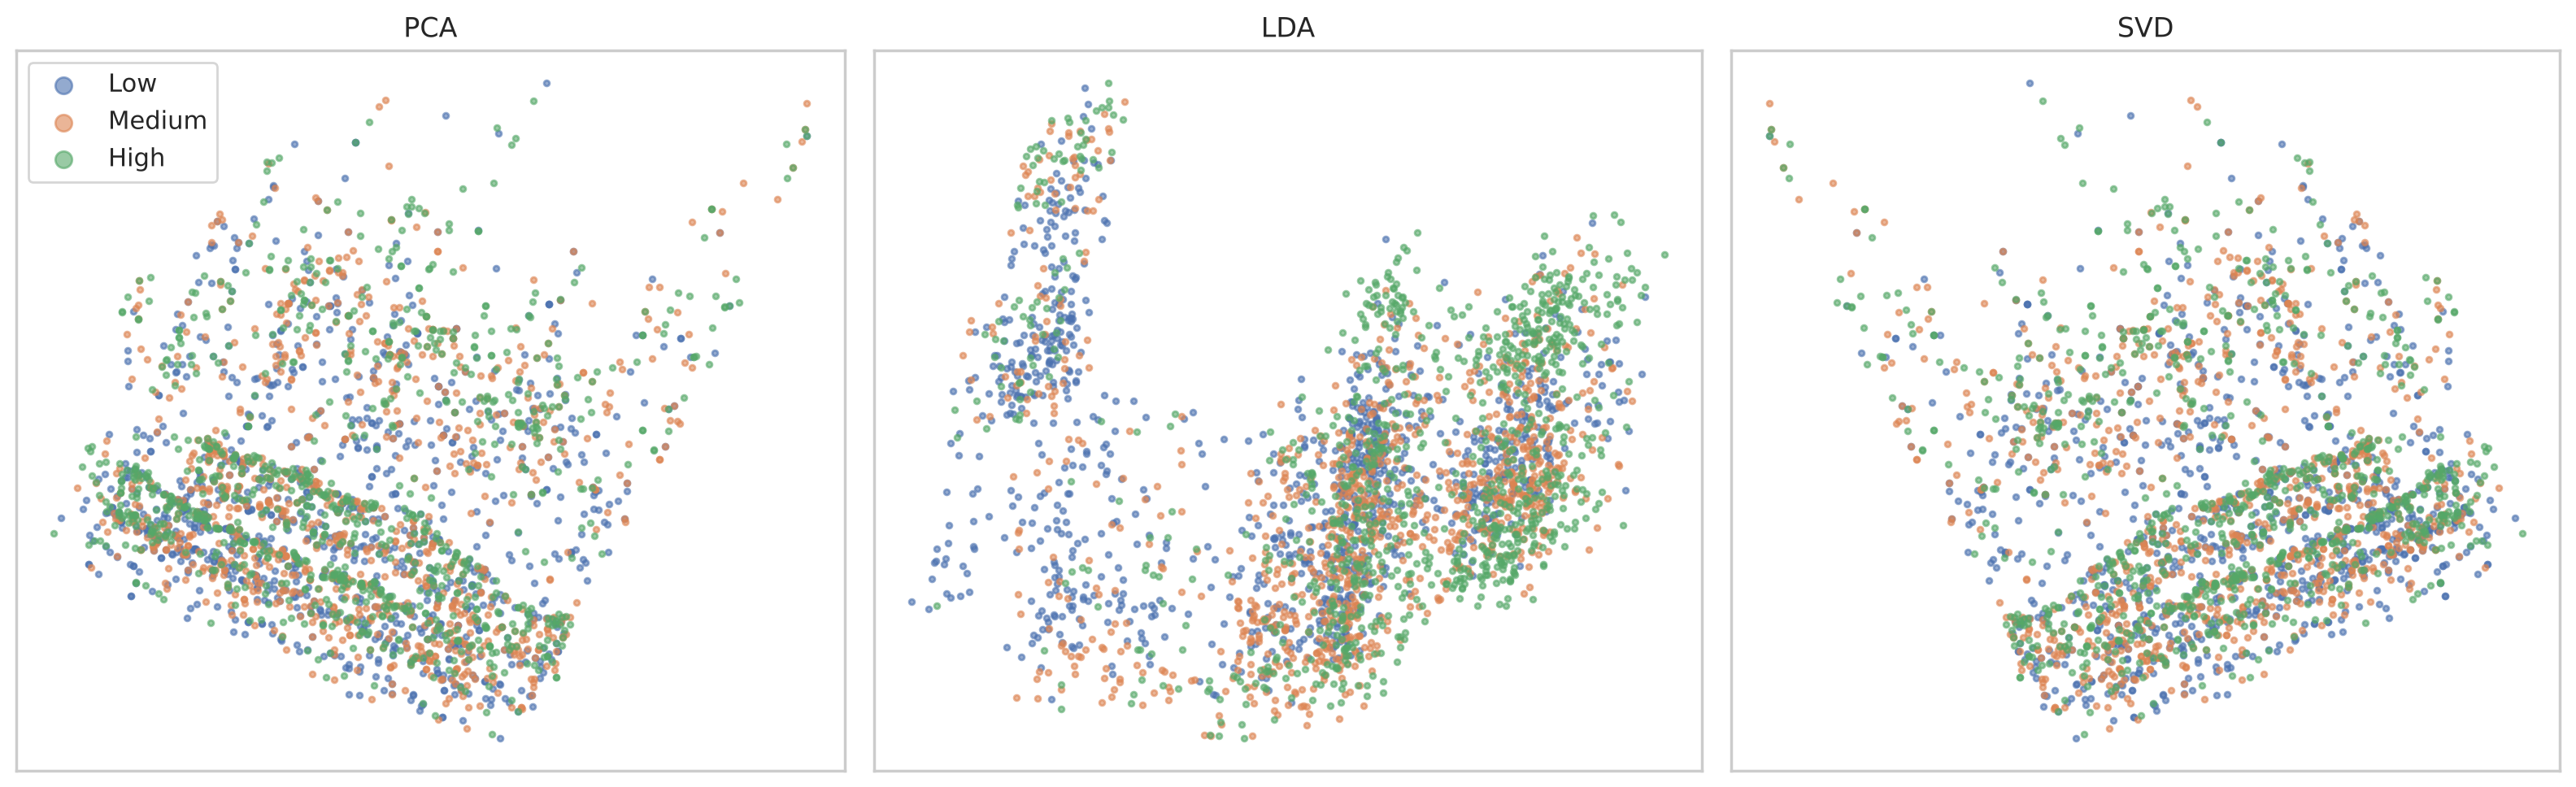
\includegraphics[width=0.92\textwidth]{figures/05_linear_embeddings.png}
\caption{Linear 2-D embeddings of the 3{,}000-point visualisation sample, coloured by the true sales class. PCA and SVD are identical up to sign; only the supervised LDA shows partial class separation.}
\label{fig:linear}
\end{figure*}

\subsection{Non-linear feature reduction}
Table~\ref{tab:emb} and Fig.~\ref{fig:allemb} compare all ten embeddings. Three different patterns appear.

\emph{Neighbourhood preservation.} t-SNE (trustworthiness 0.996) and UMAP (0.990) preserve local neighbourhoods almost perfectly, followed by our SNE implementation (0.958). The global methods --- PCA, SVD, Kernel PCA, both MDS variants and Isomap --- lie between 0.89 and 0.91, and LLE is lowest (0.841). This ranking matches theory: the neighbour-embedding family optimises exactly what trustworthiness measures, whereas distance-preserving methods trade local fidelity for global layout. In the t-SNE and UMAP maps the data split into a handful of compact islands. To find out what they represent, we trained a 5-NN classifier in each embedding to predict different labels. It recovers the store type with 99.4\% (t-SNE) and 98.8\% (UMAP) accuracy, the year with 97.8\% and 96.3\%, and the promotion era (\texttt{MarkDown\_Available}) with 99.5\% and 99.3\%, but the sales class with only 39.5\% and 38.8\%. The islands are therefore \emph{store-context} groups (type $\times$ year $\times$ promotion regime), not sales segments.

\emph{Class information.} No unsupervised embedding separates the classes well. The 5-NN accuracies lie between 35.1\% (LLE) and 39.5\% (t-SNE), all \emph{below} the 41.2\% obtained by 5-NN on the 25 standardised features themselves. All class silhouettes are slightly negative ($-0.08$ to $-0.01$), meaning that a point is on average as close to points of the other classes as to its own. Squeezing 25 noisy dimensions into two therefore loses class information, and the loss is largest for methods whose objective is global (MDS, Isomap) or fragile (LLE). LDA is the exception because it is supervised.

\emph{Method-specific behaviour.} \textbf{Kernel PCA} performed best with the smallest bandwidth tried ($\gamma=0.005$), where the RBF kernel is almost linear, and is then visually and numerically close to PCA (36.4\%). Larger $\gamma$ values produced numerically unstable eigenvectors and were discarded. \textbf{SNE} produces a looser, more uniform cloud than t-SNE --- the classic \emph{crowding problem} that motivated the heavy-tailed kernel of t-SNE~\cite{vandermaaten2008} --- and it is also by far the slowest method in our pure-NumPy implementation (44.8\,s for 1{,}500 points, against 7.9\,s for t-SNE on 3{,}000 points). \textbf{Metric and non-metric MDS} give nearly identical maps (37.4\% and 37.0\%). The rank-based non-metric variant costs 14 times more (55.2\,s versus 4.0\,s) for no benefit, which shows that the distance structure contains no monotone distortion worth modelling. \textbf{Isomap} unrolls the data into elongated filaments that follow the calendar ordering. \textbf{LLE} collapses most points onto a single line (Fig.~\ref{fig:allemb}). This is a well-known failure mode when the neighbourhood graph contains many exact duplicates: here, departments of the same store-week share every context feature, so the local reconstruction problem becomes degenerate.

\begin{table}[!t]
\caption{Quality of the 2-D embeddings (3{,}000-point training sample). kNN = 5-fold 5-NN accuracy in the embedding; reference on the 25 raw standardised features: 0.412}
\label{tab:emb}
\centering
\setlength{\tabcolsep}{4pt}
\begin{tabular}{lcccr}
\toprule
Method & kNN acc. & Trustw. & Class sil. & Time (s) \\
\midrule
\multicolumn{5}{l}{\emph{Linear}}\\
PCA & 0.371 & 0.889 & $-0.016$ & 0.002 \\
LDA (supervised) & \textbf{0.463} & 0.699 & $-0.020$ & 0.14 \\
SVD & 0.371 & 0.889 & $-0.016$ & 0.005 \\
\midrule
\multicolumn{5}{l}{\emph{Non-linear}}\\
Kernel PCA ($\gamma$=0.005) & 0.364 & 0.889 & $-0.014$ & 2.1 \\
SNE$^\dagger$ & 0.373 & 0.958 & $-0.019$ & 44.8 \\
t-SNE & 0.395 & \textbf{0.996} & $-0.024$ & 7.9 \\
UMAP & 0.388 & 0.990 & $-0.030$ & 10.8 \\
Metric MDS$^\ddagger$ & 0.374 & 0.899 & $-0.023$ & 4.0 \\
Non-metric MDS$^\ddagger$ & 0.370 & 0.900 & $-0.029$ & 55.2 \\
Isomap & 0.374 & 0.910 & $-0.043$ & 1.9 \\
LLE & 0.351 & 0.841 & $-0.079$ & 2.3 \\
\bottomrule
\multicolumn{5}{l}{\footnotesize $^\dagger$1{,}500 points, own NumPy implementation; $^\ddagger$1{,}000 points.}
\end{tabular}
\end{table}

\begin{figure*}[!t]
\centering
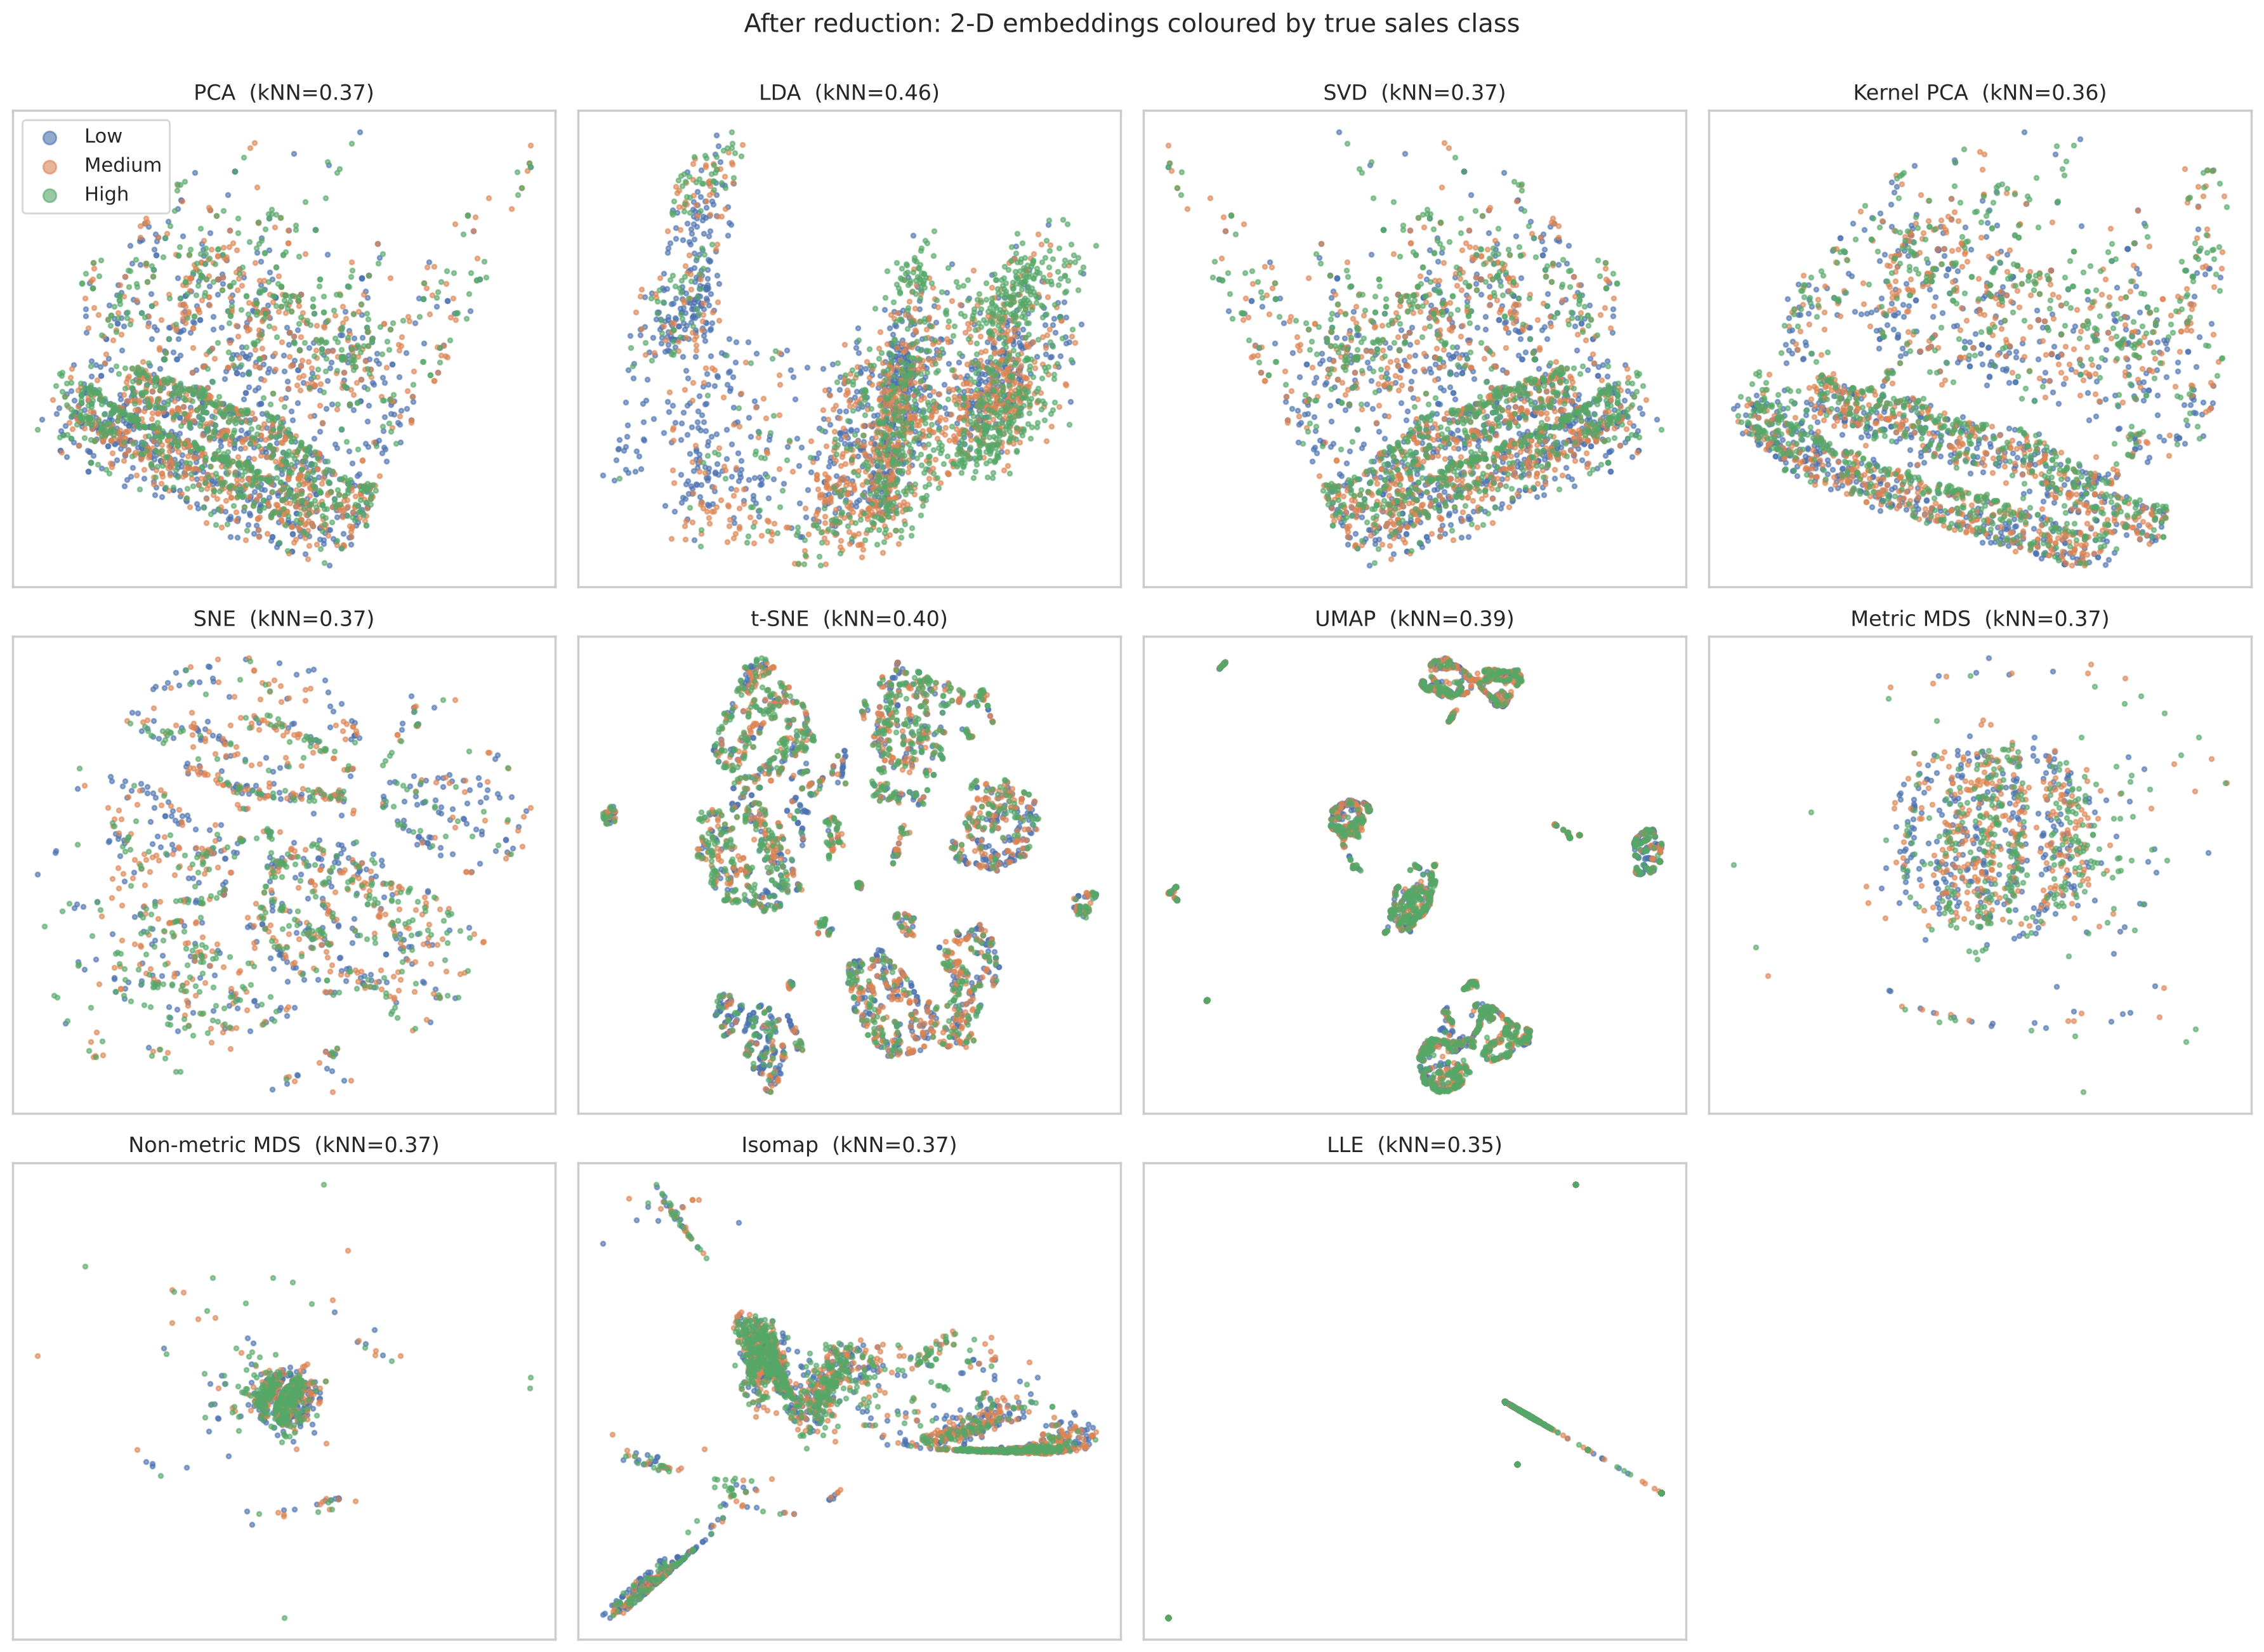
\includegraphics[width=\textwidth]{figures/06_all_embeddings.png}
\caption{After reduction: all ten 2-D embeddings coloured by the true sales class (5-NN accuracy in brackets). Neighbour-embedding methods (t-SNE, UMAP) reveal compact store-context islands, but no unsupervised method separates the sales classes.}
\label{fig:allemb}
\end{figure*}

\subsection{Clustering before and after reduction}
Table~\ref{tab:clu} and Fig.~\ref{fig:clu} report K-Means ($k=3$) in six spaces. In the original 25-D space and in the 16-D PCA space the clusters are weak (silhouette 0.13--0.14). After reduction to 2-D the silhouette rises sharply: 0.44 (PCA), 0.45 (LDA), 0.47 (t-SNE) and 0.57 (UMAP). UMAP's compact islands are exactly what K-Means rewards. The agreement with the true sales classes, however, is close to zero everywhere (ARI $\le0.018$, NMI $\le0.024$). The data clearly contain natural groups --- seasons, promotion eras, store-size tiers --- but these groups are orthogonal to the sales level of a department. This is the central negative result of the unsupervised part of the study: \emph{a high silhouette after reduction does not mean that the clusters are meaningful for the business target}, and an analyst who reads a good-looking UMAP map as ``three sales segments'' would be badly misled.

\begin{table}[!t]
\caption{K-Means ($k=3$) before and after reduction}
\label{tab:clu}
\centering
\begin{tabular}{lccc}
\toprule
Space & Silhouette & ARI & NMI \\
\midrule
Original (25-D) & 0.131 & 0.000 & 0.001 \\
PCA (16-D, 95\% var.) & 0.136 & 0.000 & 0.001 \\
PCA (2-D) & 0.437 & 0.001 & 0.001 \\
LDA (2-D) & 0.453 & \textbf{0.018} & \textbf{0.024} \\
t-SNE (2-D) & 0.473 & 0.008 & 0.008 \\
UMAP (2-D) & \textbf{0.570} & 0.009 & 0.009 \\
\bottomrule
\end{tabular}
\end{table}

\begin{figure*}[!t]
\centering
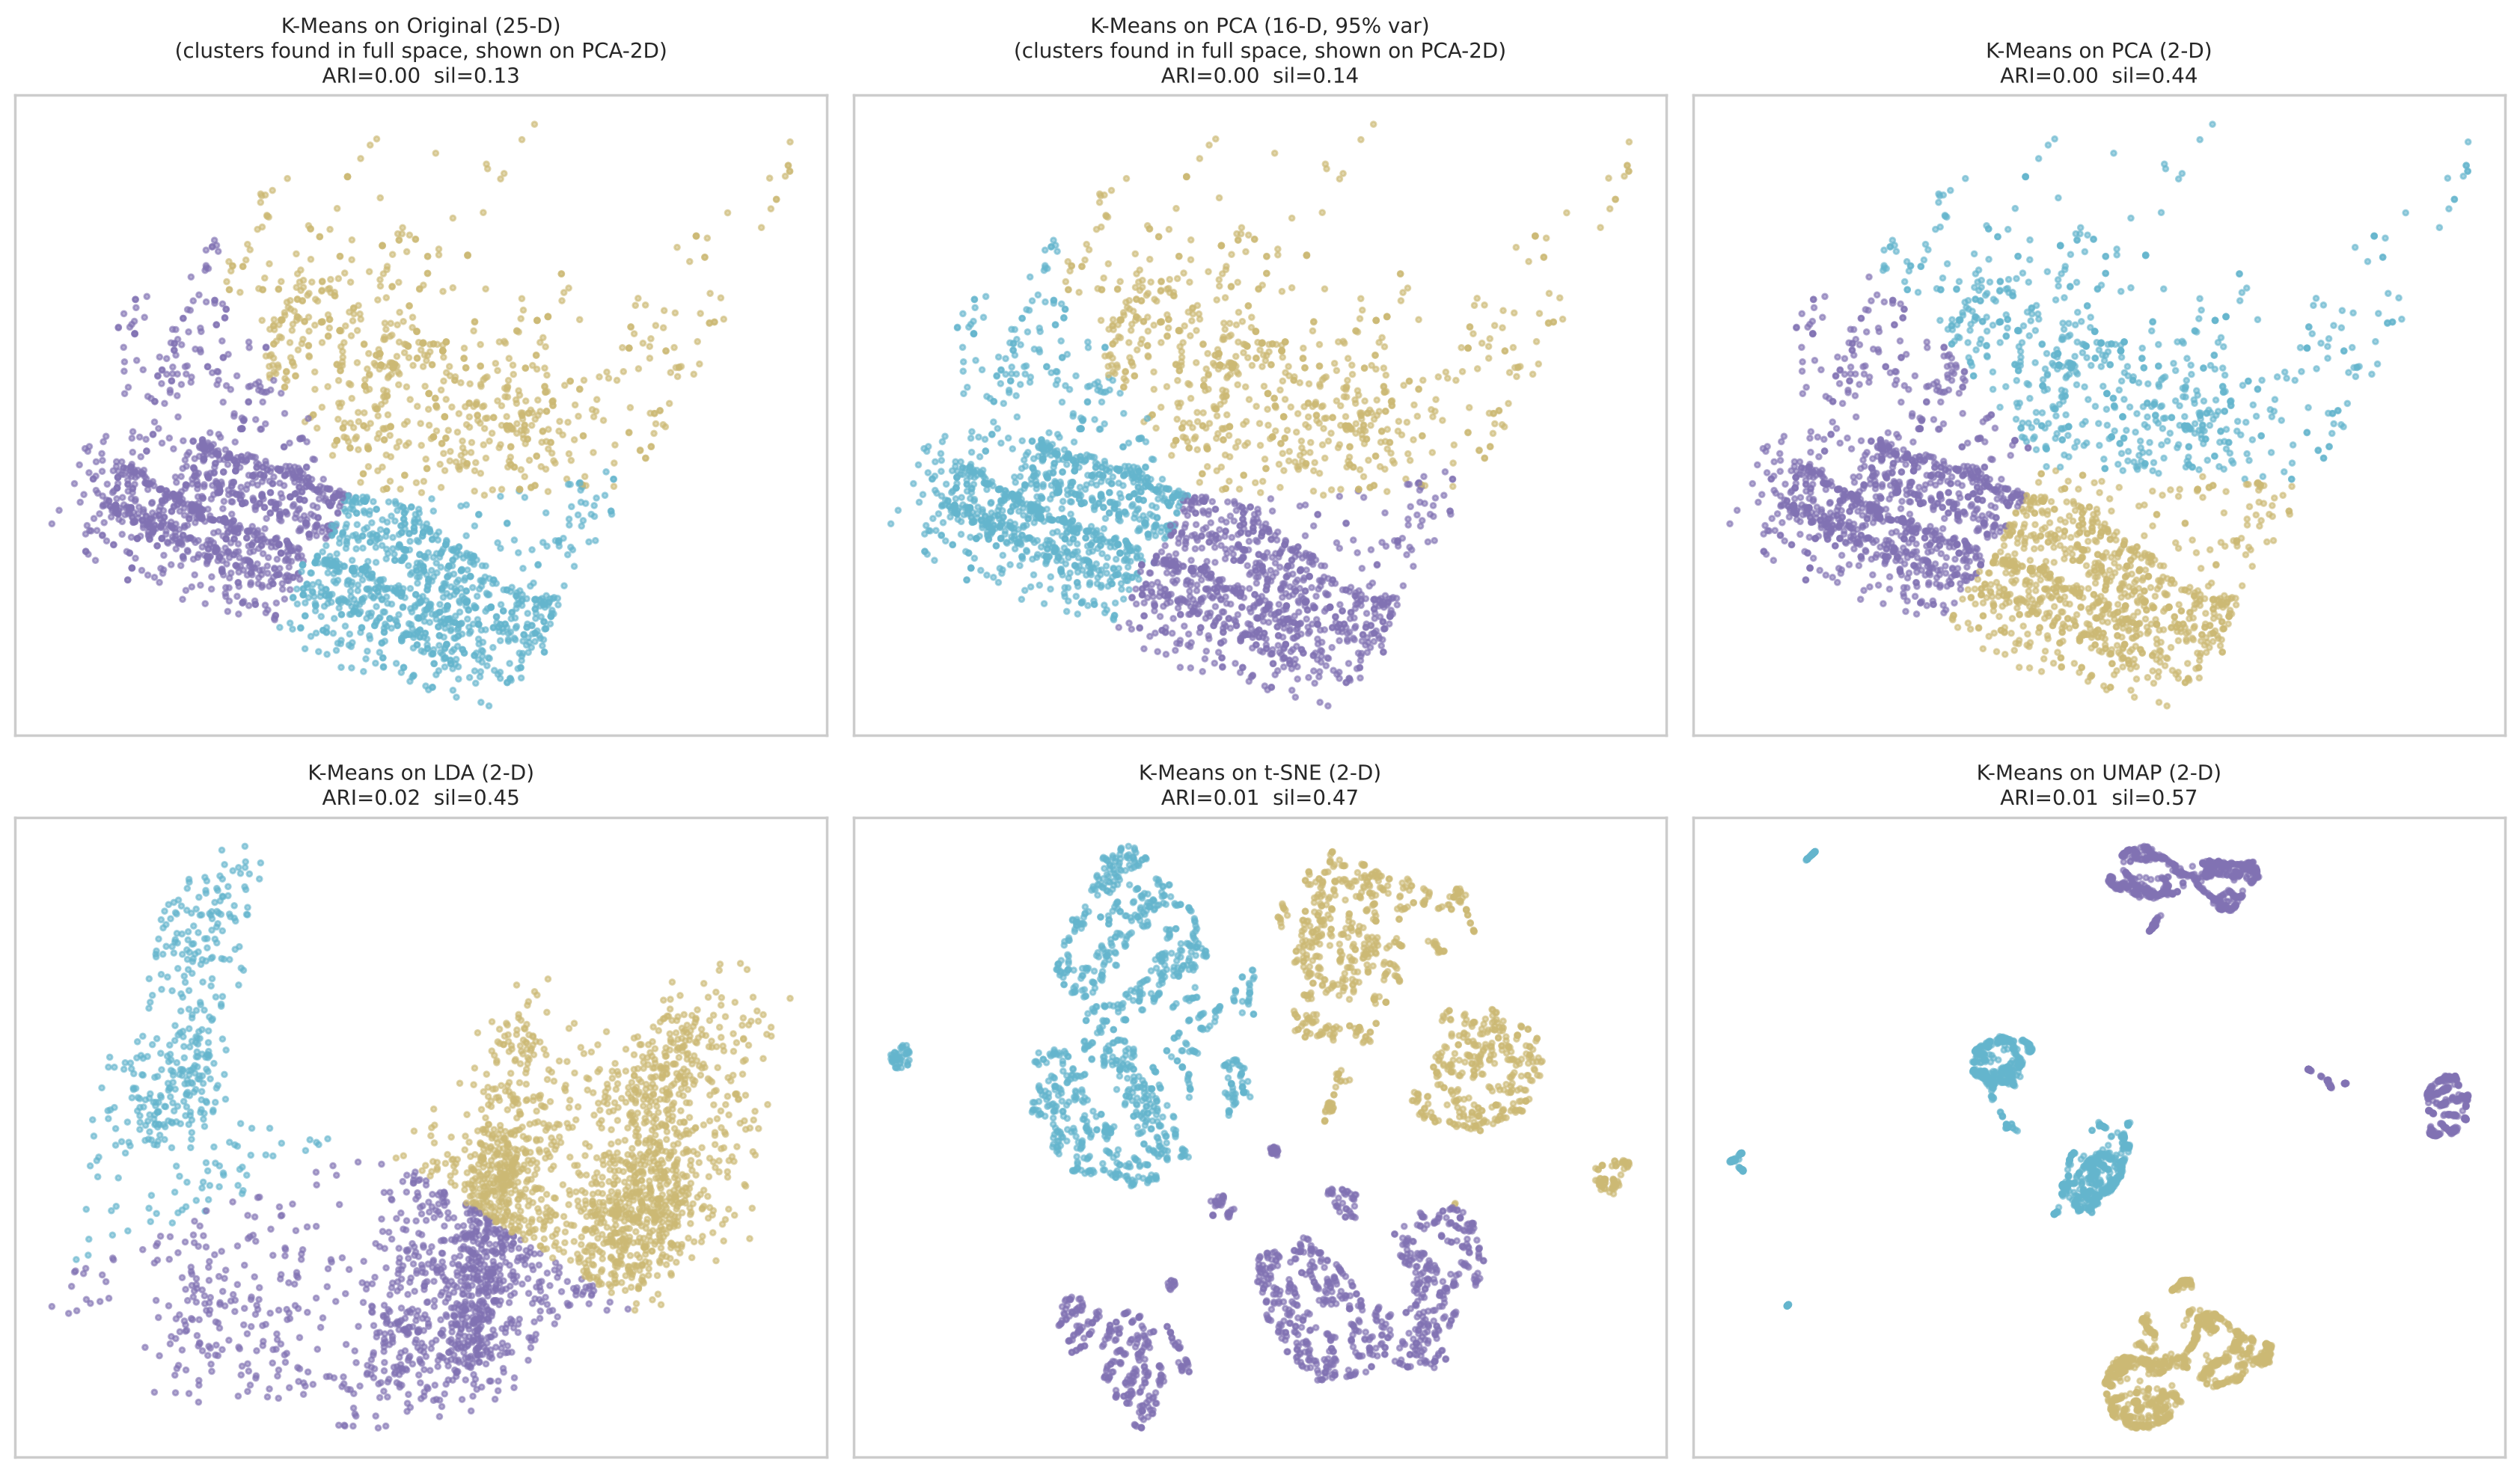
\includegraphics[width=0.92\textwidth]{figures/07_clustering_before_after.png}
\caption{K-Means clusters before (top-left, top-middle: found in the full space and shown on the PCA plane) and after reduction. The clusters become crisper after reduction (higher silhouette) but remain unrelated to the sales classes (ARI $\approx0$).}
\label{fig:clu}
\end{figure*}

\subsection{Filter feature selection}
Table~\ref{tab:filter} lists the ten best features by rank fusion and Fig.~\ref{fig:filter} shows three of the individual scores. The filters disagree in an instructive way. The linear and monotone statistics (Spearman, ANOVA-F, $\chi^2$) all rank \texttt{Size} and the store-type dummies at the top and give \texttt{Dept} only a modest score ($|\rho|=0.027$). Mutual information, which captures arbitrary dependence, ranks \texttt{Dept} first by a wide margin (MI $=0.418$ nats, almost seven times the next feature, \texttt{Store} with 0.063). Rank fusion produces a compromise that keeps \texttt{Dept} (fourth) but also keeps all three redundant type dummies, three MarkDowns and \texttt{CPI}. The variance filter flags only \texttt{MarkDown3} as near-constant (min--max variance $<0.01$), because most of its mass sits at zero after imputation. Filters are fast (under one second) but blind to redundancy and interactions --- the main reason why the filter subset is the weakest of all selected subsets in Section~\ref{sec:res:subsets}.

\begin{table}[!t]
\caption{Filter scores of the ten best features by mean rank (20k training rows)}
\label{tab:filter}
\centering
\setlength{\tabcolsep}{3pt}
\begin{tabular}{lrrrrr}
\toprule
Feature & $|\rho_S|$ & ANOVA $F$ & $\chi^2$ & MI & Rank \\
\midrule
Size & 0.270 & 900.8 & 325.3 & 0.061 & 2.00 \\
Type\_A & 0.191 & 376.6 & 354.0 & 0.018 & 3.00 \\
Type\_C & 0.148 & 317.4 & 553.1 & 0.014 & 3.75 \\
Dept & 0.027 & 82.0 & 35.6 & \textbf{0.418} & 4.75 \\
Store & 0.077 & 79.9 & 28.0 & 0.063 & 4.75 \\
Type\_B & 0.104 & 147.3 & 178.1 & 0.007 & 6.50 \\
MarkDown1 & 0.027 & 38.8 & 24.5 & 0.015 & 7.50 \\
MarkDown4 & 0.050 & 27.6 & 19.0 & 0.011 & 8.25 \\
MarkDown5 & 0.025 & 27.3 & 15.0 & 0.014 & 9.25 \\
CPI & 0.025 & 10.9 & 7.3 & 0.012 & 10.50 \\
\bottomrule
\end{tabular}
\end{table}

\begin{figure*}[!t]
\centering
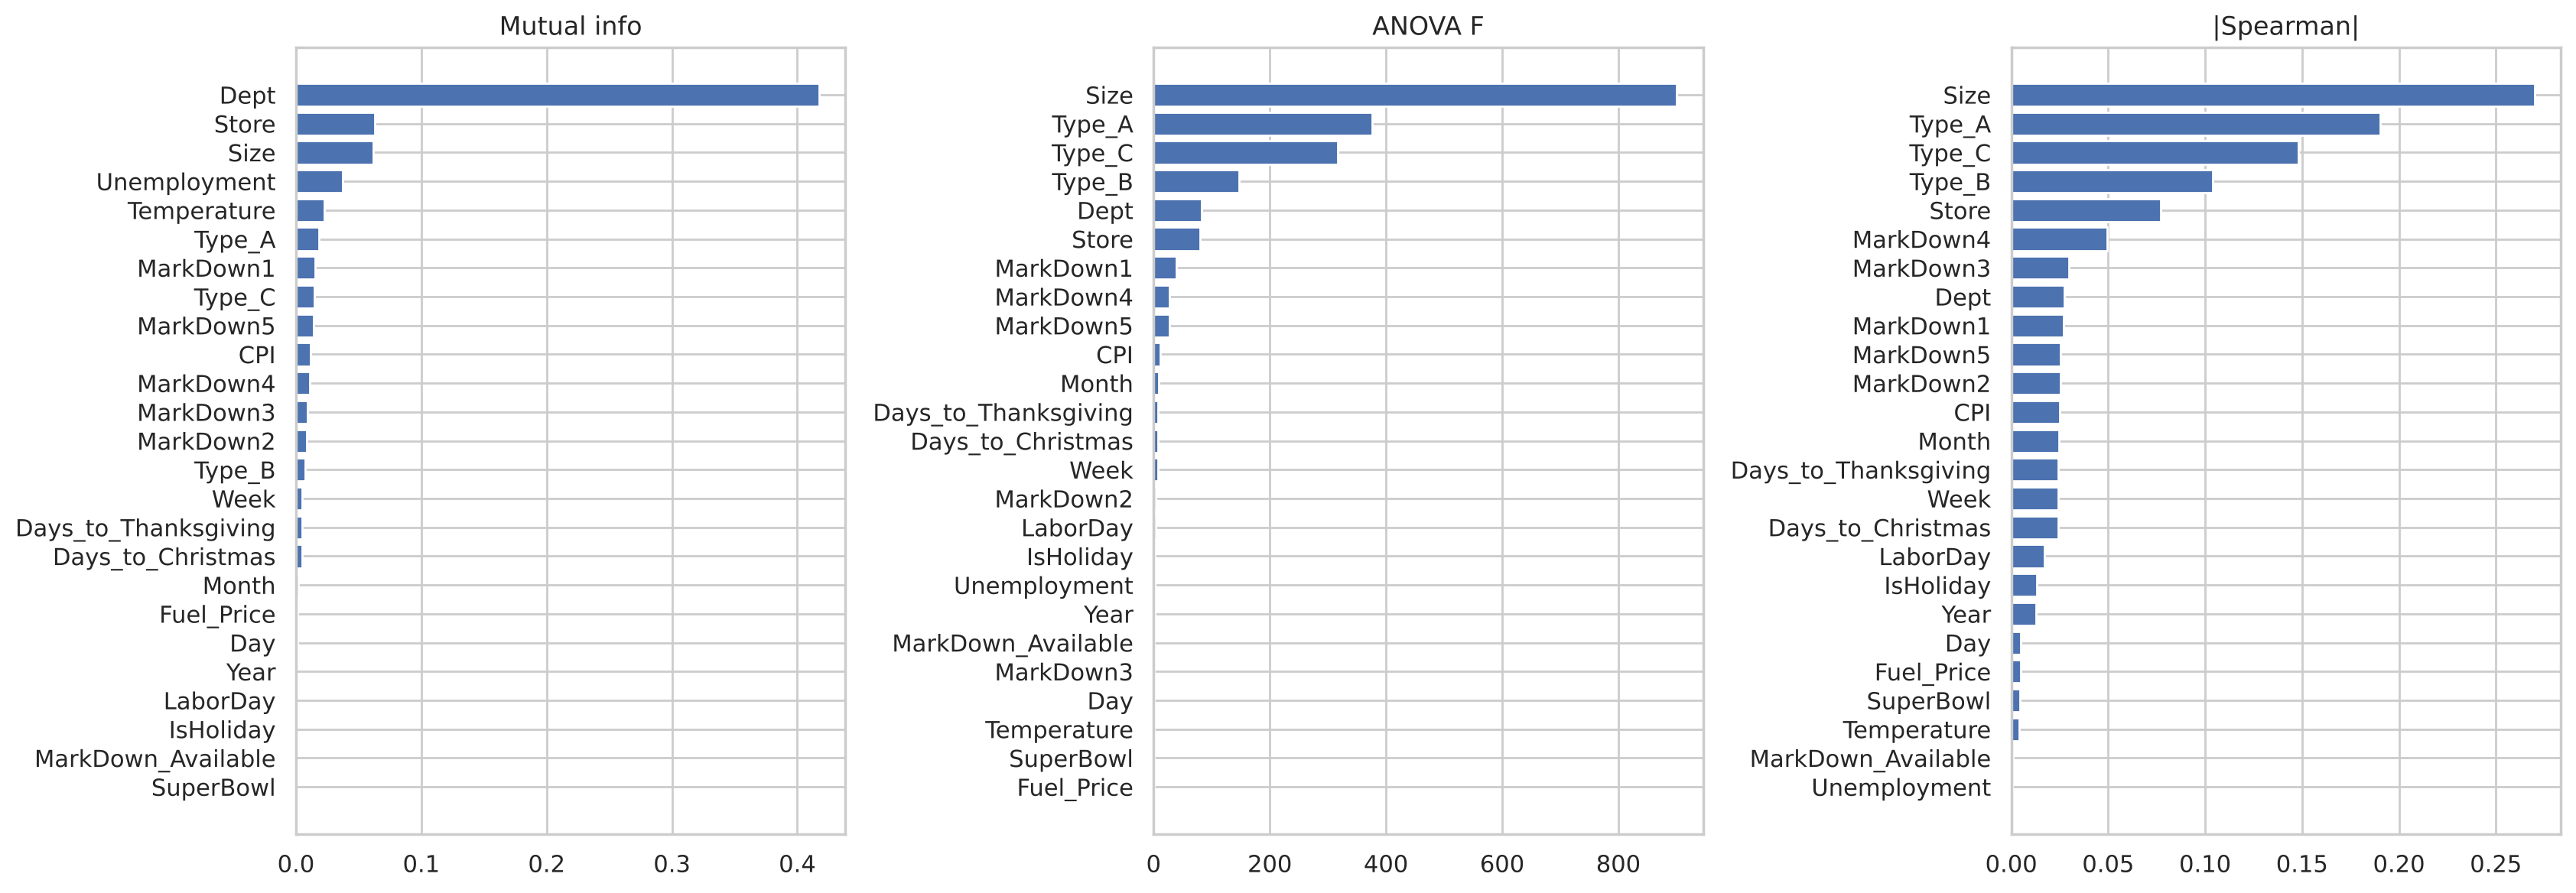
\includegraphics[width=0.95\textwidth]{figures/08_filter_scores.png}
\caption{Filter scores. Mutual information (left) is the only filter that recognises \texttt{Dept} as the dominant feature; ANOVA-F and Spearman (middle, right) favour \texttt{Size} and the store type.}
\label{fig:filter}
\end{figure*}

\subsection{Wrapper feature selection}
Each wrapper evaluates hundreds of candidate subsets with the actual learning algorithm and therefore captures interactions. All three wrappers keep the store-identity block \{\texttt{Store}, \texttt{Dept}, \texttt{Size}\} and \texttt{Week}, and they reach similar 3-fold macro-F1 on the selection sample: SFS-forward 0.871, SFS-backward 0.867 and RFE 0.866. They differ in what they add. Forward selection adds the cheap categorical context (store type, holiday flags), backward selection keeps three MarkDowns plus \texttt{CPI} and \texttt{Unemployment}, and RFE --- driven by random-forest impurity importance, which is biased towards high-cardinality continuous variables --- keeps the four economic variables and two calendar variables. Their costs differ widely: RFE took 14\,s, SFS-forward 99\,s and SFS-backward 201\,s, because backward elimination must evaluate large subsets in its first steps.

\subsection{Embedded feature selection}
The regularised logistic regressions show how much the penalty shapes the selection (Fig.~\ref{fig:emb}). With $C=0.05$, L1 sets 6 of 25 coefficient vectors to exactly zero (19 kept), Elastic-Net sets 4 to zero (21 kept), and L2, as expected, sets none to zero, so its ten largest coefficient norms are used. All three models agree on the ordering of the top features --- \texttt{Size}, \texttt{Type\_C}, \texttt{Dept}, \texttt{Type\_B}, \texttt{CPI} --- and all three reach only 44.1\% accuracy even on the data they were fitted on. This is the clearest evidence of \emph{under-fitting} in the study. A linear model cannot represent the effect of a nominal identifier such as \texttt{Dept}, so the penalty is selecting among features of a model that is itself inadequate, and the selected subsets inherit that limitation (Section~\ref{sec:res:subsets}). The gain importance of LightGBM, a non-linear embedded selector, paints a very different picture: \texttt{Dept} alone accounts for \textbf{67.0\%} of the total gain, \texttt{Size} for 14.5\% and \texttt{Store} for 4.8\%, while the 15 weakest features together contribute less than 4\%.

\begin{figure*}[!t]
\centering
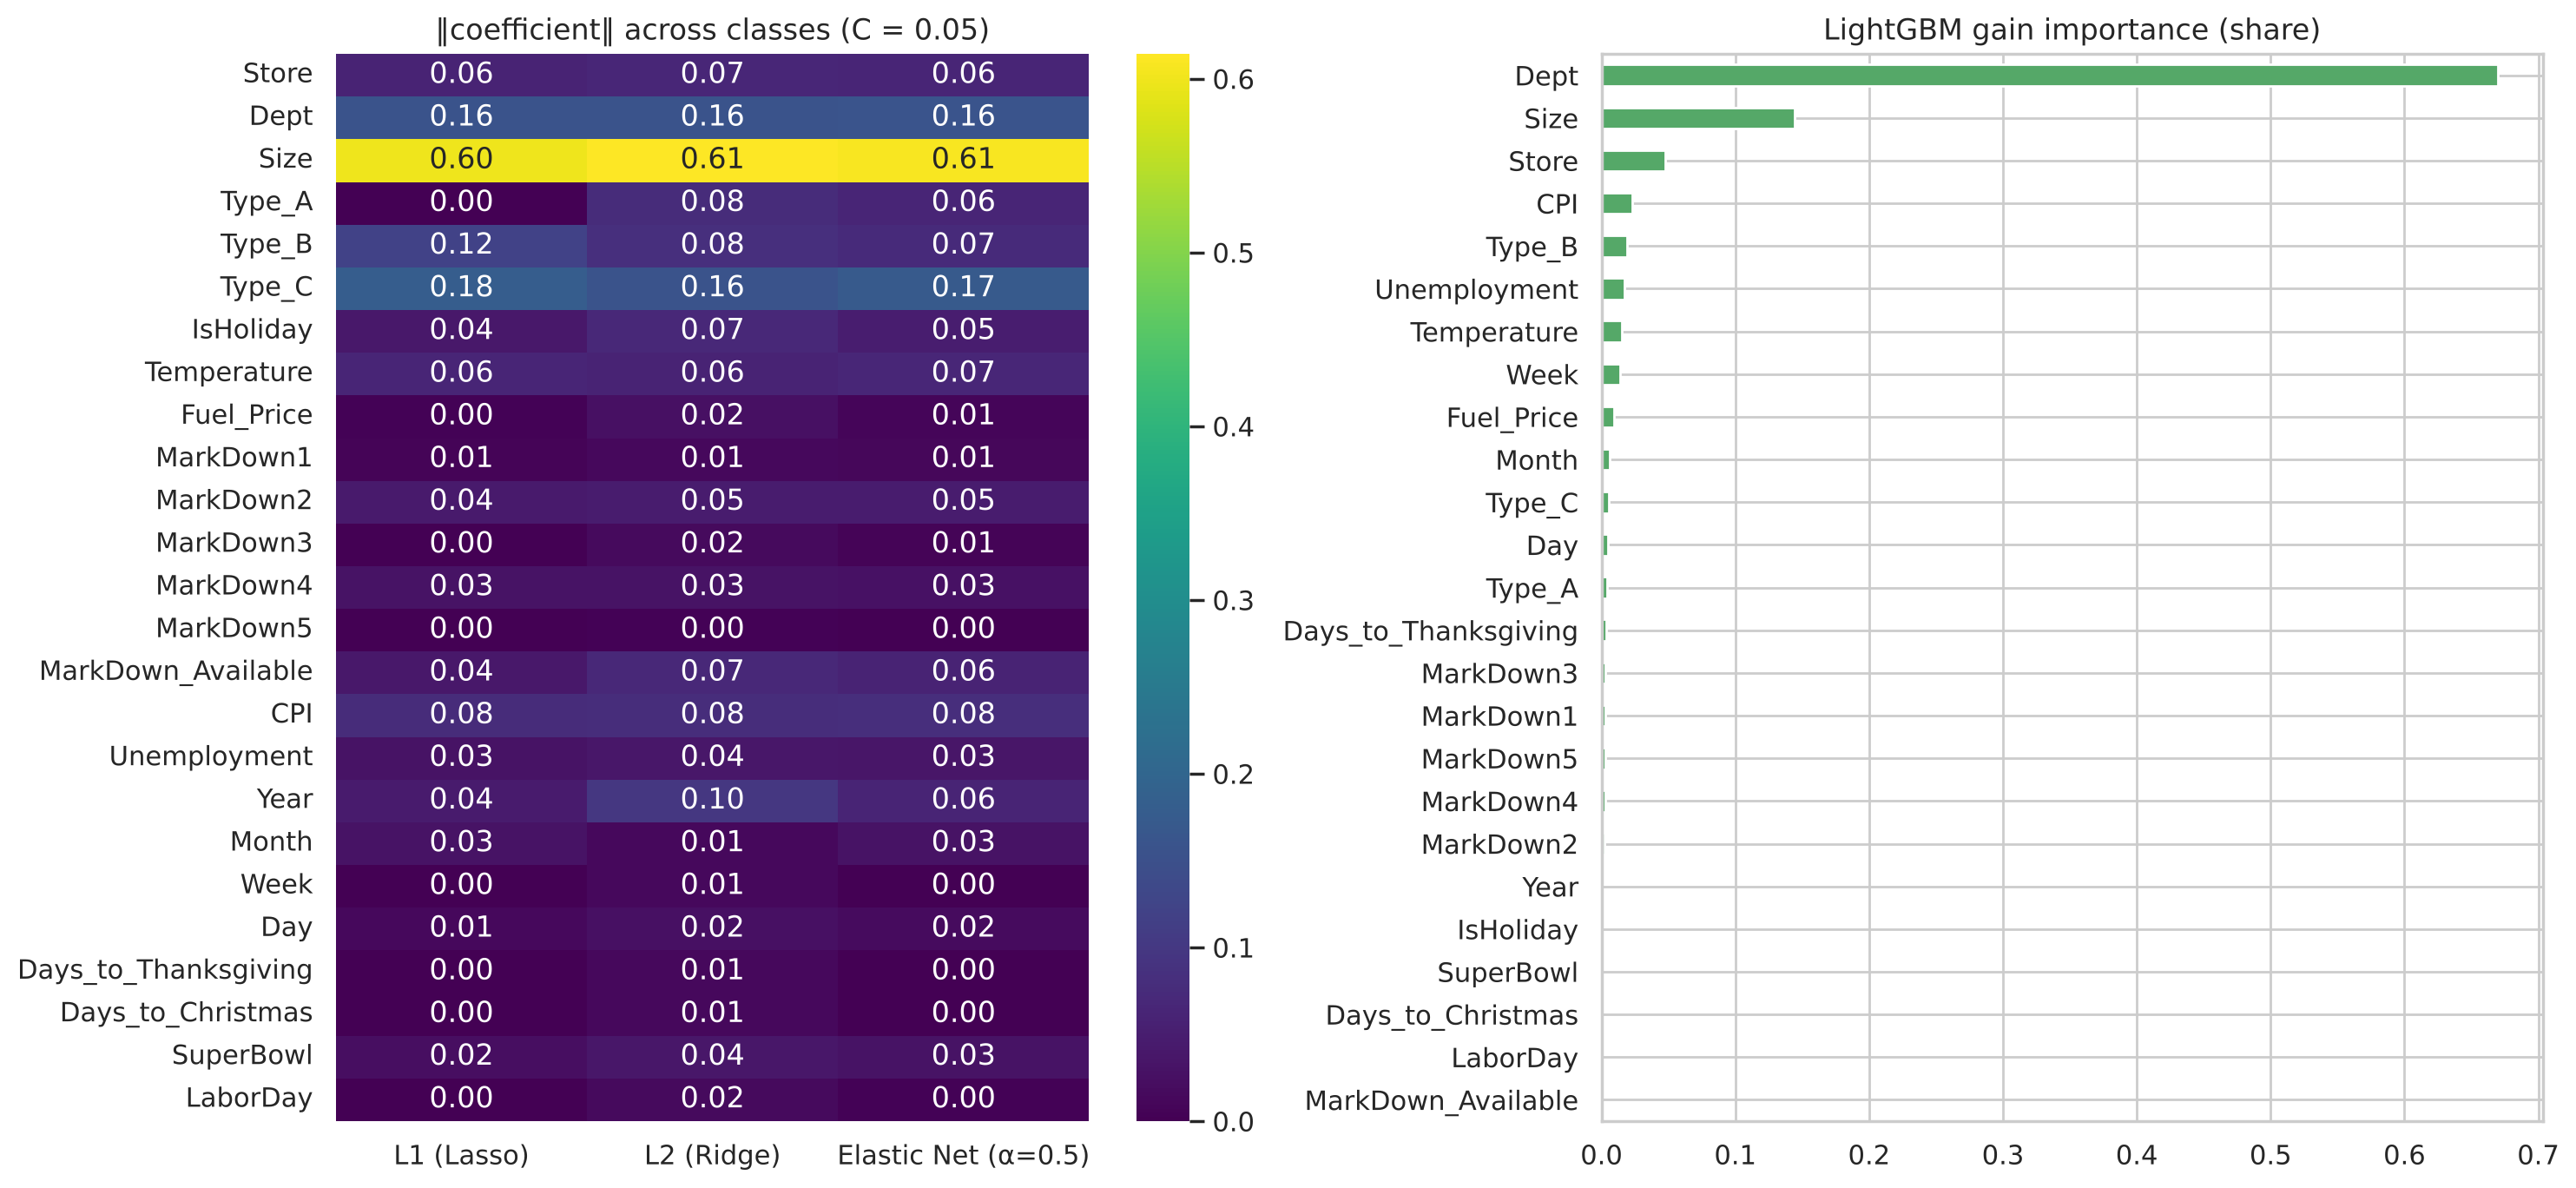
\includegraphics[width=0.9\textwidth]{figures/09_embedded.png}
\caption{Embedded selection. Left: norm of the multinomial logistic-regression coefficients under L1, L2 and Elastic-Net penalties (zero = removed). Right: LightGBM gain share, dominated by \texttt{Dept}.}
\label{fig:emb}
\end{figure*}

\subsection{Metaheuristic feature selection}
Table~\ref{tab:meta} and Fig.~\ref{fig:meta} summarise the three metaheuristics, which all optimise the size-penalised fitness of Eq.~(\ref{eq:fitness}). All three converge to very similar regions of the search space and keep the same core \{\texttt{Store}, \texttt{Dept}, \texttt{Size}, \texttt{Type\_B}\}, which is a strong sign that this core is genuinely sufficient. The GA keeps \textbf{6 features} (core + \texttt{CPI} + \texttt{Week}). BPSO keeps 9 (core + \texttt{CPI}, \texttt{IsHoliday} and three holiday-distance variables). SA keeps only \textbf{5} (core + \texttt{Days\_to\_Thanksgiving}). On the selection sample SA attains the best fitness (0.869) and F1 (0.873), followed by the GA (0.867 / 0.872) and BPSO (0.863 / 0.870). The differences are within the noise of a 3-fold estimate.

The convergence curves (Fig.~\ref{fig:meta}) show the typical behaviour of the three algorithms. The GA improves in a few large jumps during its first generations, when crossover recombines good building blocks, and then stabilises. BPSO improves steadily as the swarm contracts around the global best. SA starts from a random mask and climbs slowly, with occasional accepted downhill moves while the temperature is high. Thanks to fitness caching, the numbers of unique subsets actually evaluated were 331 (GA), 400 (BPSO) and 248 (SA), costing 193\,s, 242\,s and 151\,s. That is roughly the cost of backward SFS, but the search yields subsets two to four times smaller.

\begin{table}[!t]
\caption{Metaheuristic feature selection (fitness of Eq.~(\ref{eq:fitness}), $\lambda=0.02$; 3-fold macro-F1 on 20k training rows)}
\label{tab:meta}
\centering
\setlength{\tabcolsep}{3.5pt}
\begin{tabular}{lccccr}
\toprule
Algorithm & \#feat. & F1 & Fitness & Evals & Time (s) \\
\midrule
GA & 6 & 0.872 & 0.867 & 331 & 193 \\
Binary PSO & 9 & 0.870 & 0.863 & 400 & 242 \\
Simulated Annealing & \textbf{5} & \textbf{0.873} & \textbf{0.869} & 248 & 151 \\
\bottomrule
\end{tabular}
\vspace{2pt}
\begin{tabular}{p{8.1cm}}
\footnotesize GA: Store, Dept, Size, Type\_B, CPI, Week.\; BPSO: Store, Dept, Size, Type\_B, IsHoliday, CPI, Days\_to\_Thanksgiving, SuperBowl, LaborDay.\; SA: Store, Dept, Size, Type\_B, Days\_to\_Thanksgiving.
\end{tabular}
\end{table}

\begin{figure}[!t]
\centering
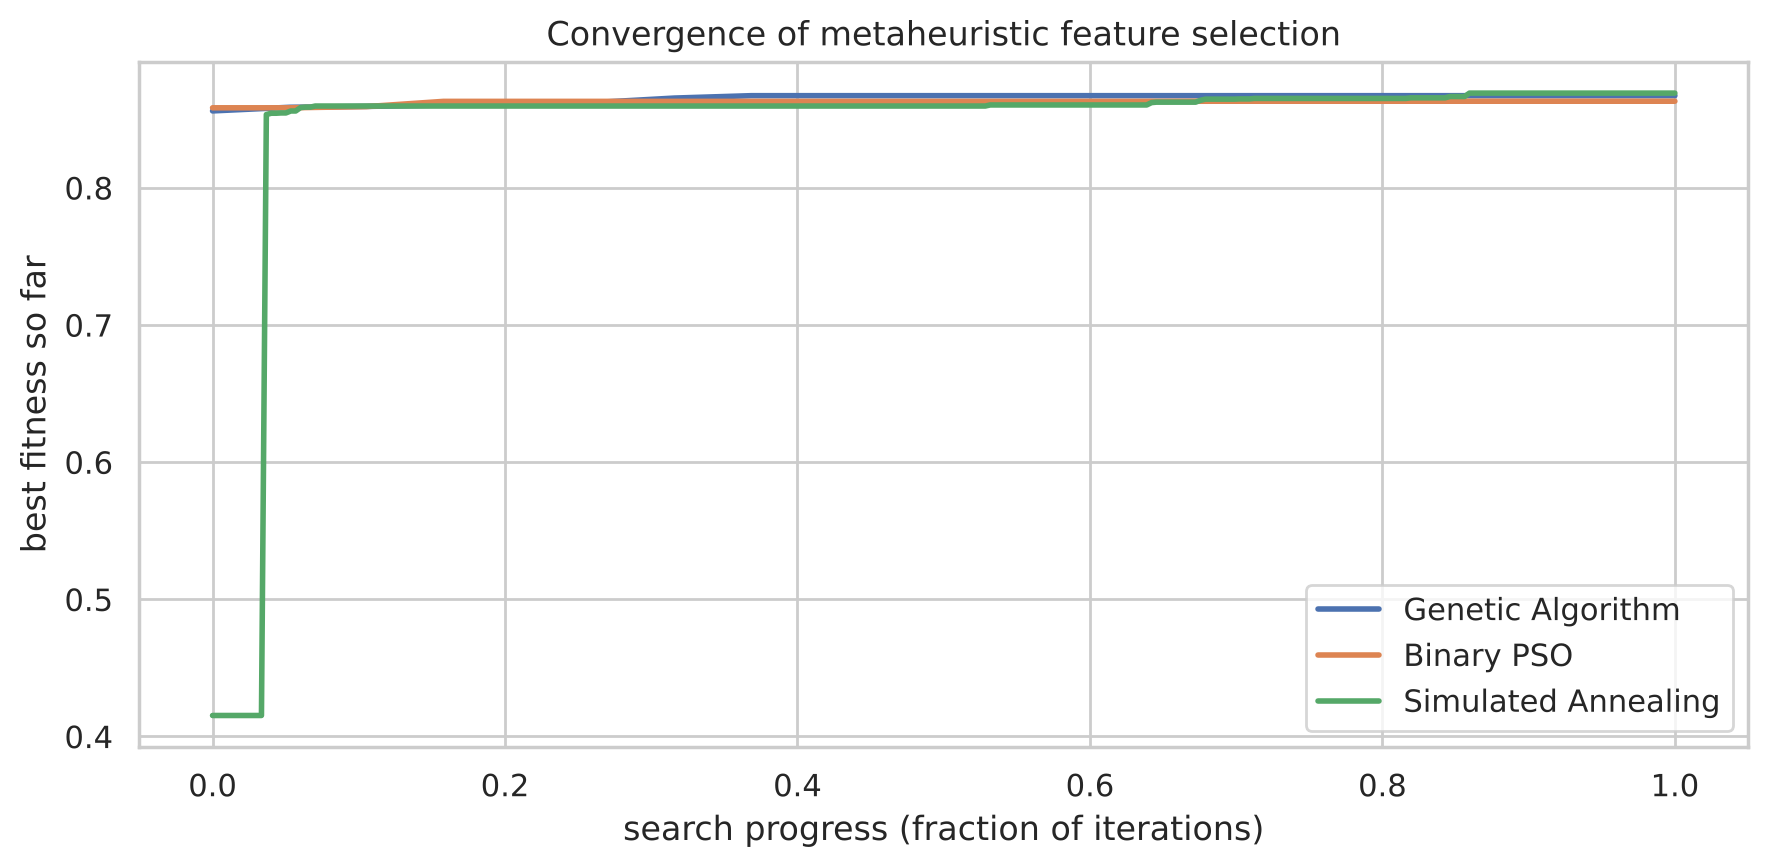
\includegraphics[width=\columnwidth]{figures/10_metaheuristic_convergence.png}
\caption{Convergence of the best fitness for GA, BPSO and SA (x-axis normalised to the fraction of iterations).}
\label{fig:meta}
\end{figure}

\subsection{Consensus across selection methods}
Fig.~\ref{fig:freq} counts how often each feature is chosen by the eleven selectors. \texttt{Store}, \texttt{Dept} and \texttt{Size} are chosen by all eleven, \texttt{Type\_B} by ten and \texttt{CPI} by nine. At the other end, \texttt{Days\_to\_Christmas} is never chosen --- it is a perfect linear copy of \texttt{Days\_to\_Thanksgiving} within each year --- and \texttt{MarkDown3} and \texttt{MarkDown5} are each chosen twice. This consensus provides a robust, method-independent answer to the question ``which variables matter'': the \emph{identity and size of the store-department} first, the macro-economic context a distant second, and the promotions and holiday flags hardly at all once the identity is known.

\begin{figure}[!t]
\centering
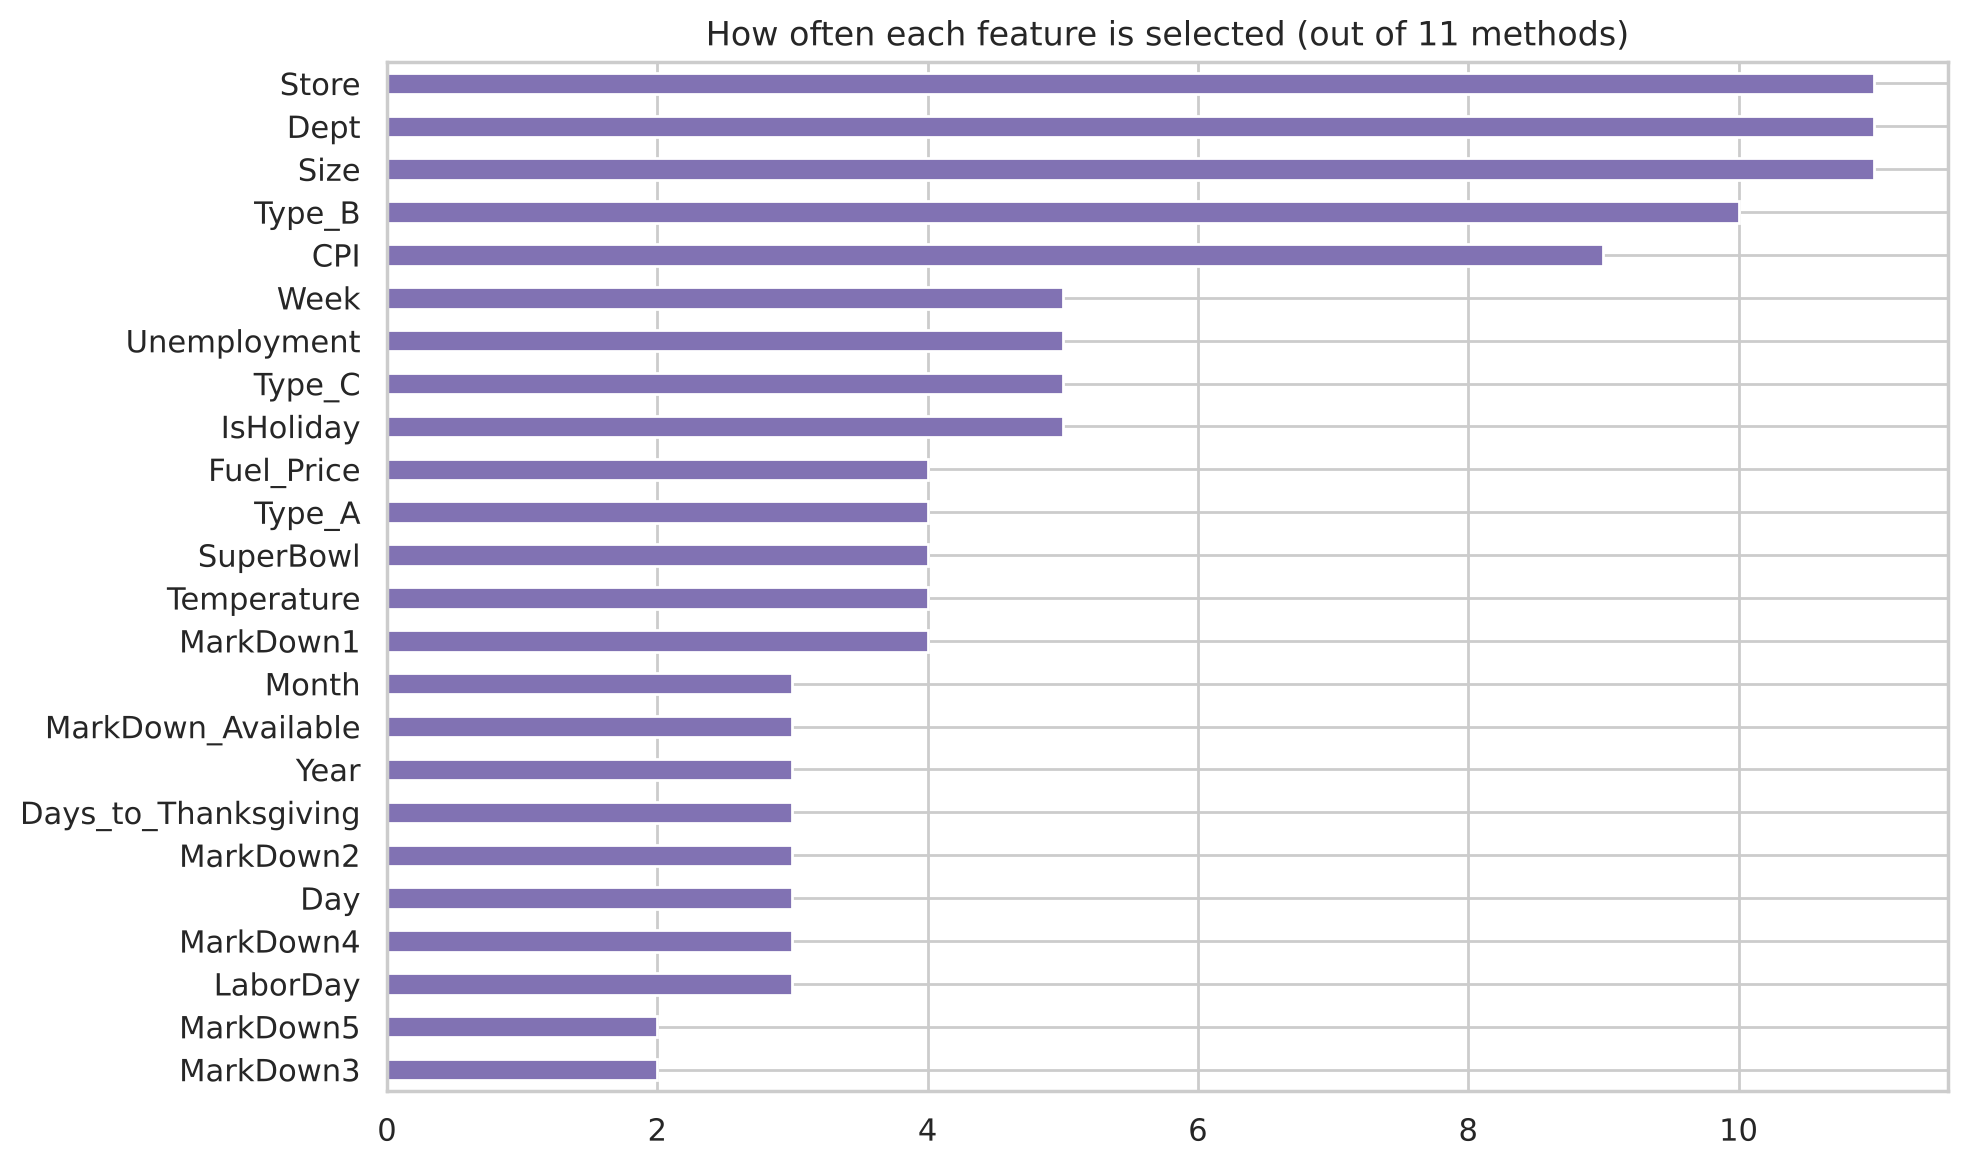
\includegraphics[width=\columnwidth]{figures/11_selection_frequency.png}
\caption{Selection frequency of each feature across the eleven selection methods.}
\label{fig:freq}
\end{figure}

\subsection{Selection before reduction}\label{sec:res:ras}
The negative result for the embeddings raises a natural question: is the weak class structure intrinsic, or is it caused by the noisy context variables, which dominate Euclidean distances? To answer it we repeated PCA, LDA, t-SNE and UMAP on the same 3{,}000 points using only the six GA-selected features (Table~\ref{tab:ras}, Fig.~\ref{fig:ras}). The effect is large for the unsupervised methods. The 5-NN accuracy rises from 37.1\% to \textbf{50.5\%} for PCA (+13.4 points), from 39.5\% to \textbf{51.5\%} for t-SNE (+12.0) and from 38.8\% to \textbf{50.0\%} for UMAP (+11.2), and trustworthiness also improves (t-SNE 0.999, UMAP 0.998, PCA 0.938). LDA is unchanged (46.3\% $\to$ 46.1\%) because, being supervised, it already down-weights irrelevant directions. K-Means still does not recover the classes (ARI $\le0.03$). Even with clean inputs, the sales level depends on department identity in a way that no compact geometric cluster captures.

The practical lesson is that \emph{feature selection should precede feature reduction} when the goal is a class-aware low-dimensional view of noisy tabular data. Unsupervised reduction treats every input dimension as equally important and cannot tell signal from noise on its own.

\begin{table}[!t]
\caption{Reduction after GA selection: 5-NN accuracy and trustworthiness on all 25 features vs.\ the 6 GA features}
\label{tab:ras}
\centering
\begin{tabular}{lcccc}
\toprule
 & \multicolumn{2}{c}{kNN accuracy} & & \\
\cmidrule{2-3}
Method & All 25 & GA 6 & $\Delta$ & Trustw.\ (GA) \\
\midrule
PCA & 0.371 & 0.505 & $+0.134$ & 0.938 \\
LDA & 0.463 & 0.461 & $-0.002$ & 0.891 \\
t-SNE & 0.395 & \textbf{0.515} & $+0.120$ & 0.999 \\
UMAP & 0.388 & 0.500 & $+0.112$ & 0.998 \\
\bottomrule
\end{tabular}
\end{table}

\begin{figure*}[!t]
\centering
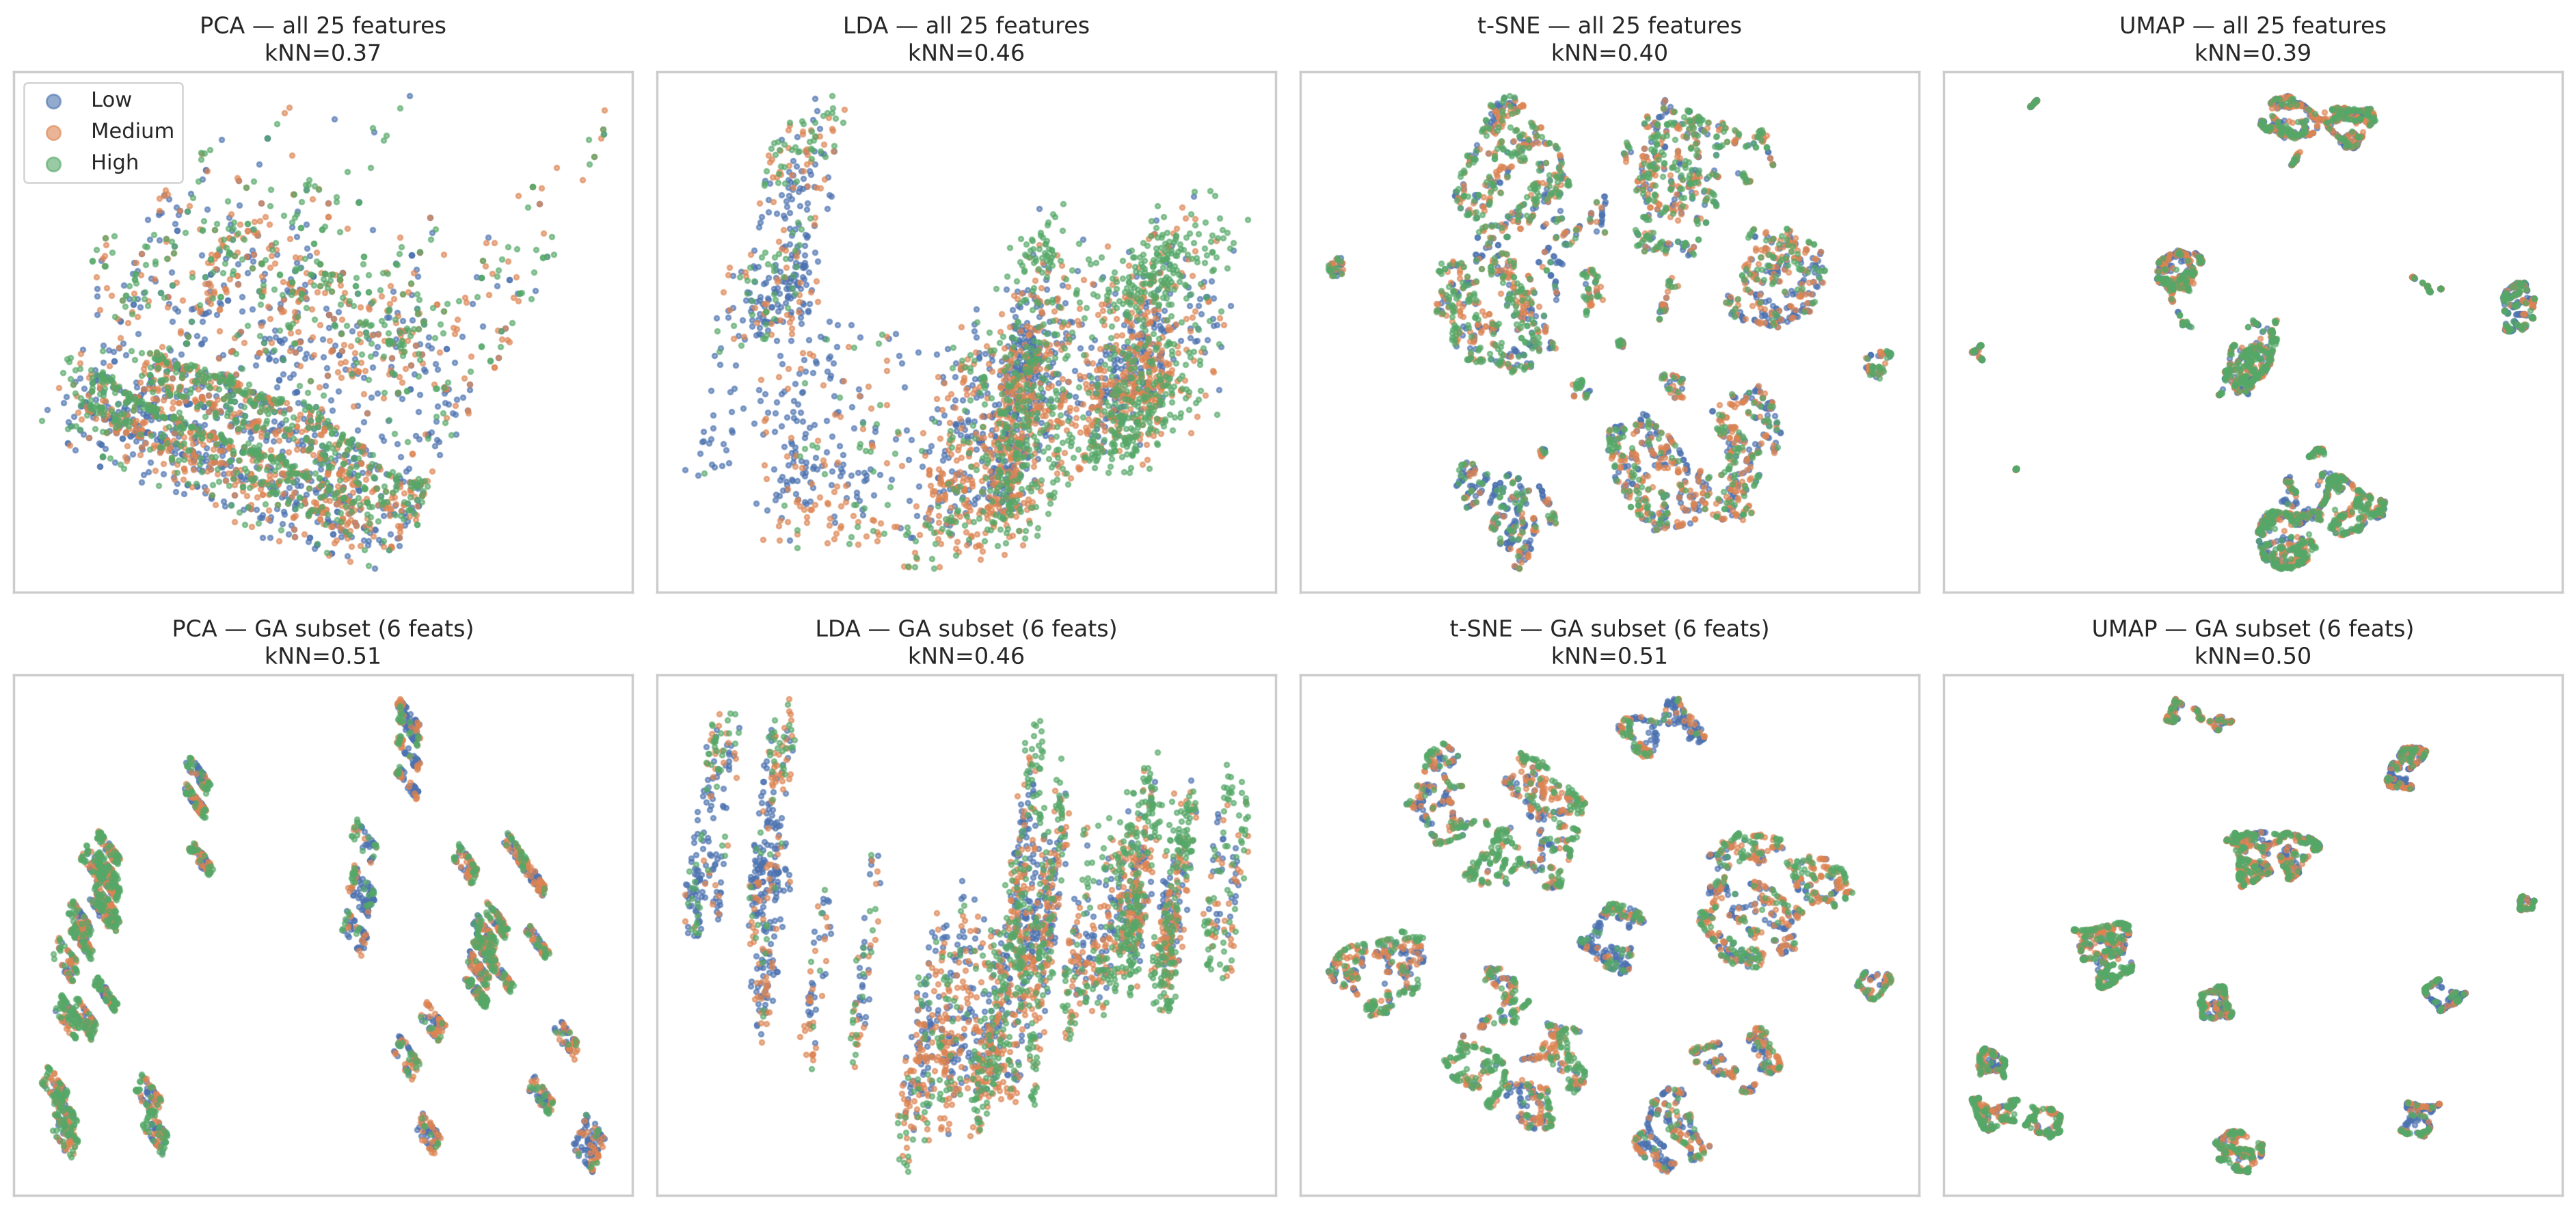
\includegraphics[width=\textwidth]{figures/17_reduction_after_selection.png}
\caption{The same 3{,}000 points embedded from all 25 features (top) and from the 6 GA-selected features (bottom). Removing noisy context variables before reduction gives markedly more class-coherent neighbourhoods.}
\label{fig:ras}
\end{figure*}

\subsection{Classification models: hold-out results}\label{sec:res:models}
Table~\ref{tab:hold} reports all requested metrics on the 20\% test split, sorted by macro-F1. Because the classes are balanced, macro precision, recall and F1 are almost equal to accuracy for every model.

The nine models fall into three clearly separated tiers. \textbf{Gradient boosting} is the best tier: LightGBM reaches \textbf{93.44\% accuracy} (error rate 6.56\%), macro-F1 0.934 and ROC-AUC 0.991, with XGBoost a close second (93.18\%, AUC 0.990). The \textbf{unpruned decision tree} forms the second tier on its own (90.18\%), but its ROC-AUC is much lower (0.926) because a fully grown tree outputs almost hard 0/1 probabilities that rank poorly. The third tier contains every model that cannot exploit \texttt{Dept} as a nominal identifier: the MLP (68.98\%), the random forest (67.08\%), extra trees (60.08\%), $k$-NN (50.80\%), Gaussian naive Bayes (46.16\%) and logistic regression (44.39\%). These are only 11--36 points above the 33.3\% chance level.

\begin{table*}[!t]
\caption{Hold-out evaluation (80{,}000 train / 20{,}000 test rows, all 25 features). Precision, recall and F1 are macro-averaged; ROC-AUC is one-vs-rest macro. Gap = train $-$ test accuracy}
\label{tab:hold}
\centering
\begin{tabular}{lcccccccccl}
\toprule
Model & Train acc. & Test acc. & Error rate & Precision & Recall & F1 & ROC-AUC & Gap & Fit (s) & Diagnosis \\
\midrule
LightGBM & 0.9929 & \textbf{0.9344} & \textbf{0.0656} & \textbf{0.9344} & \textbf{0.9344} & \textbf{0.9344} & \textbf{0.9906} & 0.059 & 9.2 & Slight over-fit \\
XGBoost & 0.9874 & 0.9318 & 0.0682 & 0.9319 & 0.9319 & 0.9318 & 0.9899 & 0.056 & 7.7 & Slight over-fit \\
Decision Tree & 1.0000 & 0.9018 & 0.0981 & 0.9018 & 0.9019 & 0.9018 & 0.9264 & 0.098 & 0.6 & Over-fitting \\
MLP & 0.7260 & 0.6898 & 0.3102 & 0.6870 & 0.6898 & 0.6870 & 0.8524 & 0.036 & 61.7 & Under-fitting \\
Random Forest & 0.9246 & 0.6708 & 0.3293 & 0.6706 & 0.6708 & 0.6701 & 0.8496 & 0.254 & 7.4 & Over-fitting \\
Extra Trees & 0.9102 & 0.6008 & 0.3992 & 0.5981 & 0.6009 & 0.5989 & 0.7883 & 0.309 & 4.9 & Over-fitting \\
KNN ($k$=15) & 0.5916 & 0.5080 & 0.4920 & 0.5065 & 0.5081 & 0.5055 & 0.6939 & 0.084 & 0.03 & Over- \& under-fit \\
Gaussian NB & 0.4560 & 0.4616 & 0.5384 & 0.4609 & 0.4617 & 0.4601 & 0.6380 & $-0.006$ & 0.06 & Under-fitting \\
Logistic Regression & 0.4412 & 0.4439 & 0.5561 & 0.4509 & 0.4439 & 0.4434 & 0.6309 & $-0.003$ & 0.2 & Under-fitting \\
\bottomrule
\end{tabular}
\end{table*}

\subsection{K-fold cross-validation}
Table~\ref{tab:cv} gives the stratified 5-fold results on the full 100k sample and Fig.~\ref{fig:cvbox} shows the fold-wise accuracies. The CV means agree with the hold-out results to within 0.2 percentage points for every model except the MLP. This confirms that the single 80/20 split is representative and that the ranking is stable. LightGBM's average accuracy is \textbf{93.42\% $\pm$ 0.20\%}, and its worst fold (93.12\%) is still better than XGBoost's mean (93.06\%). The fold-to-fold standard deviation is tiny ($\le$0.5 points) for every model except the MLP ($\pm$2.35 points). Its accuracy ranges from 63.2\% to 69.4\% depending on the fold, a sign of an unstable optimisation driven by early stopping on a small validation fraction rather than of a data effect.

\begin{table}[!t]
\caption{Stratified 5-fold cross-validation on the 100k sample (mean $\pm$ std)}
\label{tab:cv}
\centering
\setlength{\tabcolsep}{3pt}
\begin{tabular}{lccc}
\toprule
Model & Accuracy & Macro-F1 & ROC-AUC \\
\midrule
LightGBM & \textbf{0.9342}$\pm$0.0020 & \textbf{0.9343}$\pm$0.0020 & \textbf{0.9906} \\
XGBoost & 0.9306$\pm$0.0013 & 0.9307$\pm$0.0013 & 0.9898 \\
Decision Tree & 0.9042$\pm$0.0014 & 0.9042$\pm$0.0013 & 0.9282 \\
Random Forest & 0.6699$\pm$0.0019 & 0.6695$\pm$0.0018 & 0.8492 \\
MLP & 0.6645$\pm$0.0235 & 0.6606$\pm$0.0228 & 0.8361 \\
Extra Trees & 0.5953$\pm$0.0050 & 0.5936$\pm$0.0049 & 0.7855 \\
KNN ($k$=15) & 0.5091$\pm$0.0029 & 0.5070$\pm$0.0029 & 0.6915 \\
Gaussian NB & 0.4570$\pm$0.0034 & 0.4548$\pm$0.0054 & 0.6347 \\
Logistic Reg. & 0.4410$\pm$0.0007 & 0.4403$\pm$0.0006 & 0.6294 \\
\bottomrule
\end{tabular}
\end{table}

\begin{figure}[!t]
\centering
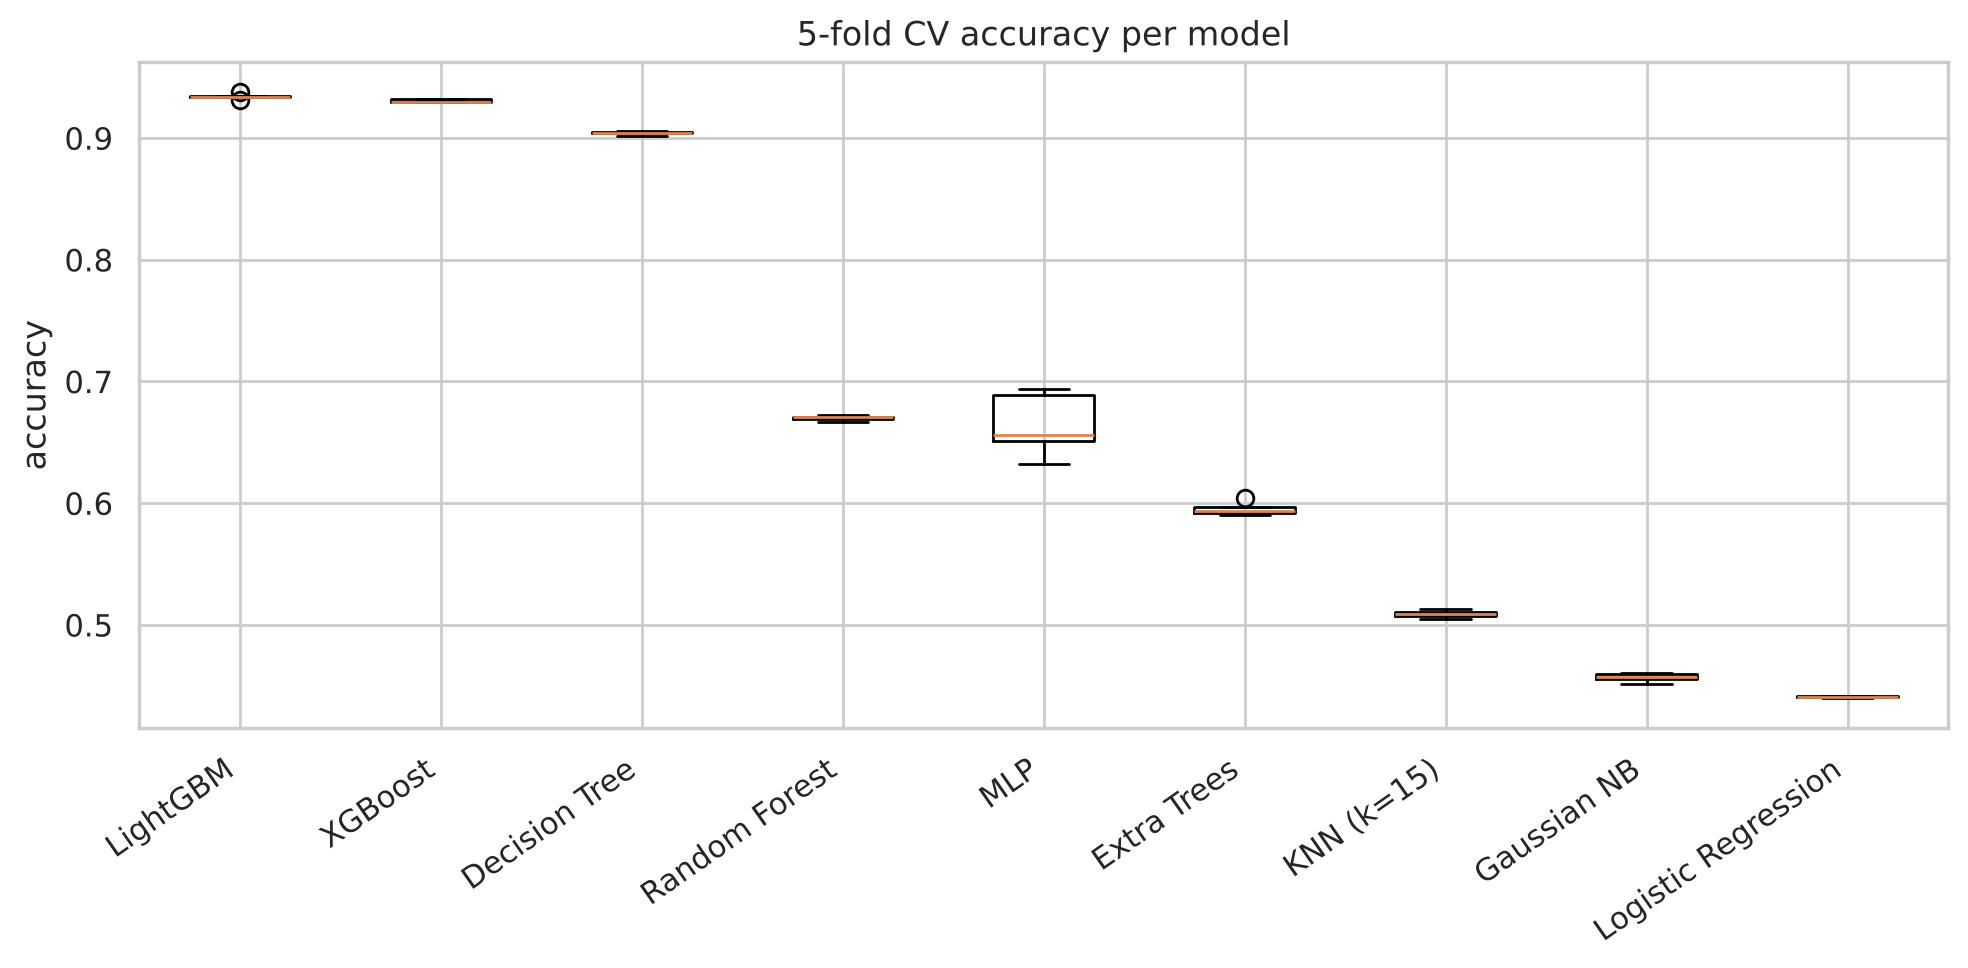
\includegraphics[width=\columnwidth]{figures/12_cv_boxplot.png}
\caption{Fold-wise 5-fold CV accuracy. Only the MLP shows a large spread.}
\label{fig:cvbox}
\end{figure}

\subsection{Confusion matrices}
Fig.~\ref{fig:cm} shows the row-normalised test confusion matrices of six models, and Table~\ref{tab:cmint} gives the per-class figures. For \textbf{LightGBM} the per-class recalls are 95.3\% (Low), 90.1\% (Medium) and 94.9\% (High). The Medium class is the hardest because it borders both other classes, while Low and High each have only one neighbour. Of LightGBM's 1{,}312 errors, the most frequent is a true Medium predicted as Low (383 cases), and only \textbf{7 errors (0.5\%) are ``far'' errors} between Low and High. The model's mistakes are therefore almost exclusively near-threshold confusions between adjacent levels, the least costly kind of error for staffing or replenishment decisions. The pattern is the same for XGBoost (9 far errors) and the decision tree (23).

For the under-fitting linear models the picture is the opposite. Logistic regression commits 11{,}122 errors, of which 3{,}094 (\textbf{27.8\%}) are far Low$\leftrightarrow$High errors, and its most common confusion is a true Medium predicted as High (2{,}698 cases). Its Medium recall is 37.2\%, barely above chance. Gaussian naive Bayes behaves similarly (26.9\% far errors). Such models do not merely blur the class boundaries; they lack any usable notion of the ordering of sales levels.

\begin{figure*}[!t]
\centering
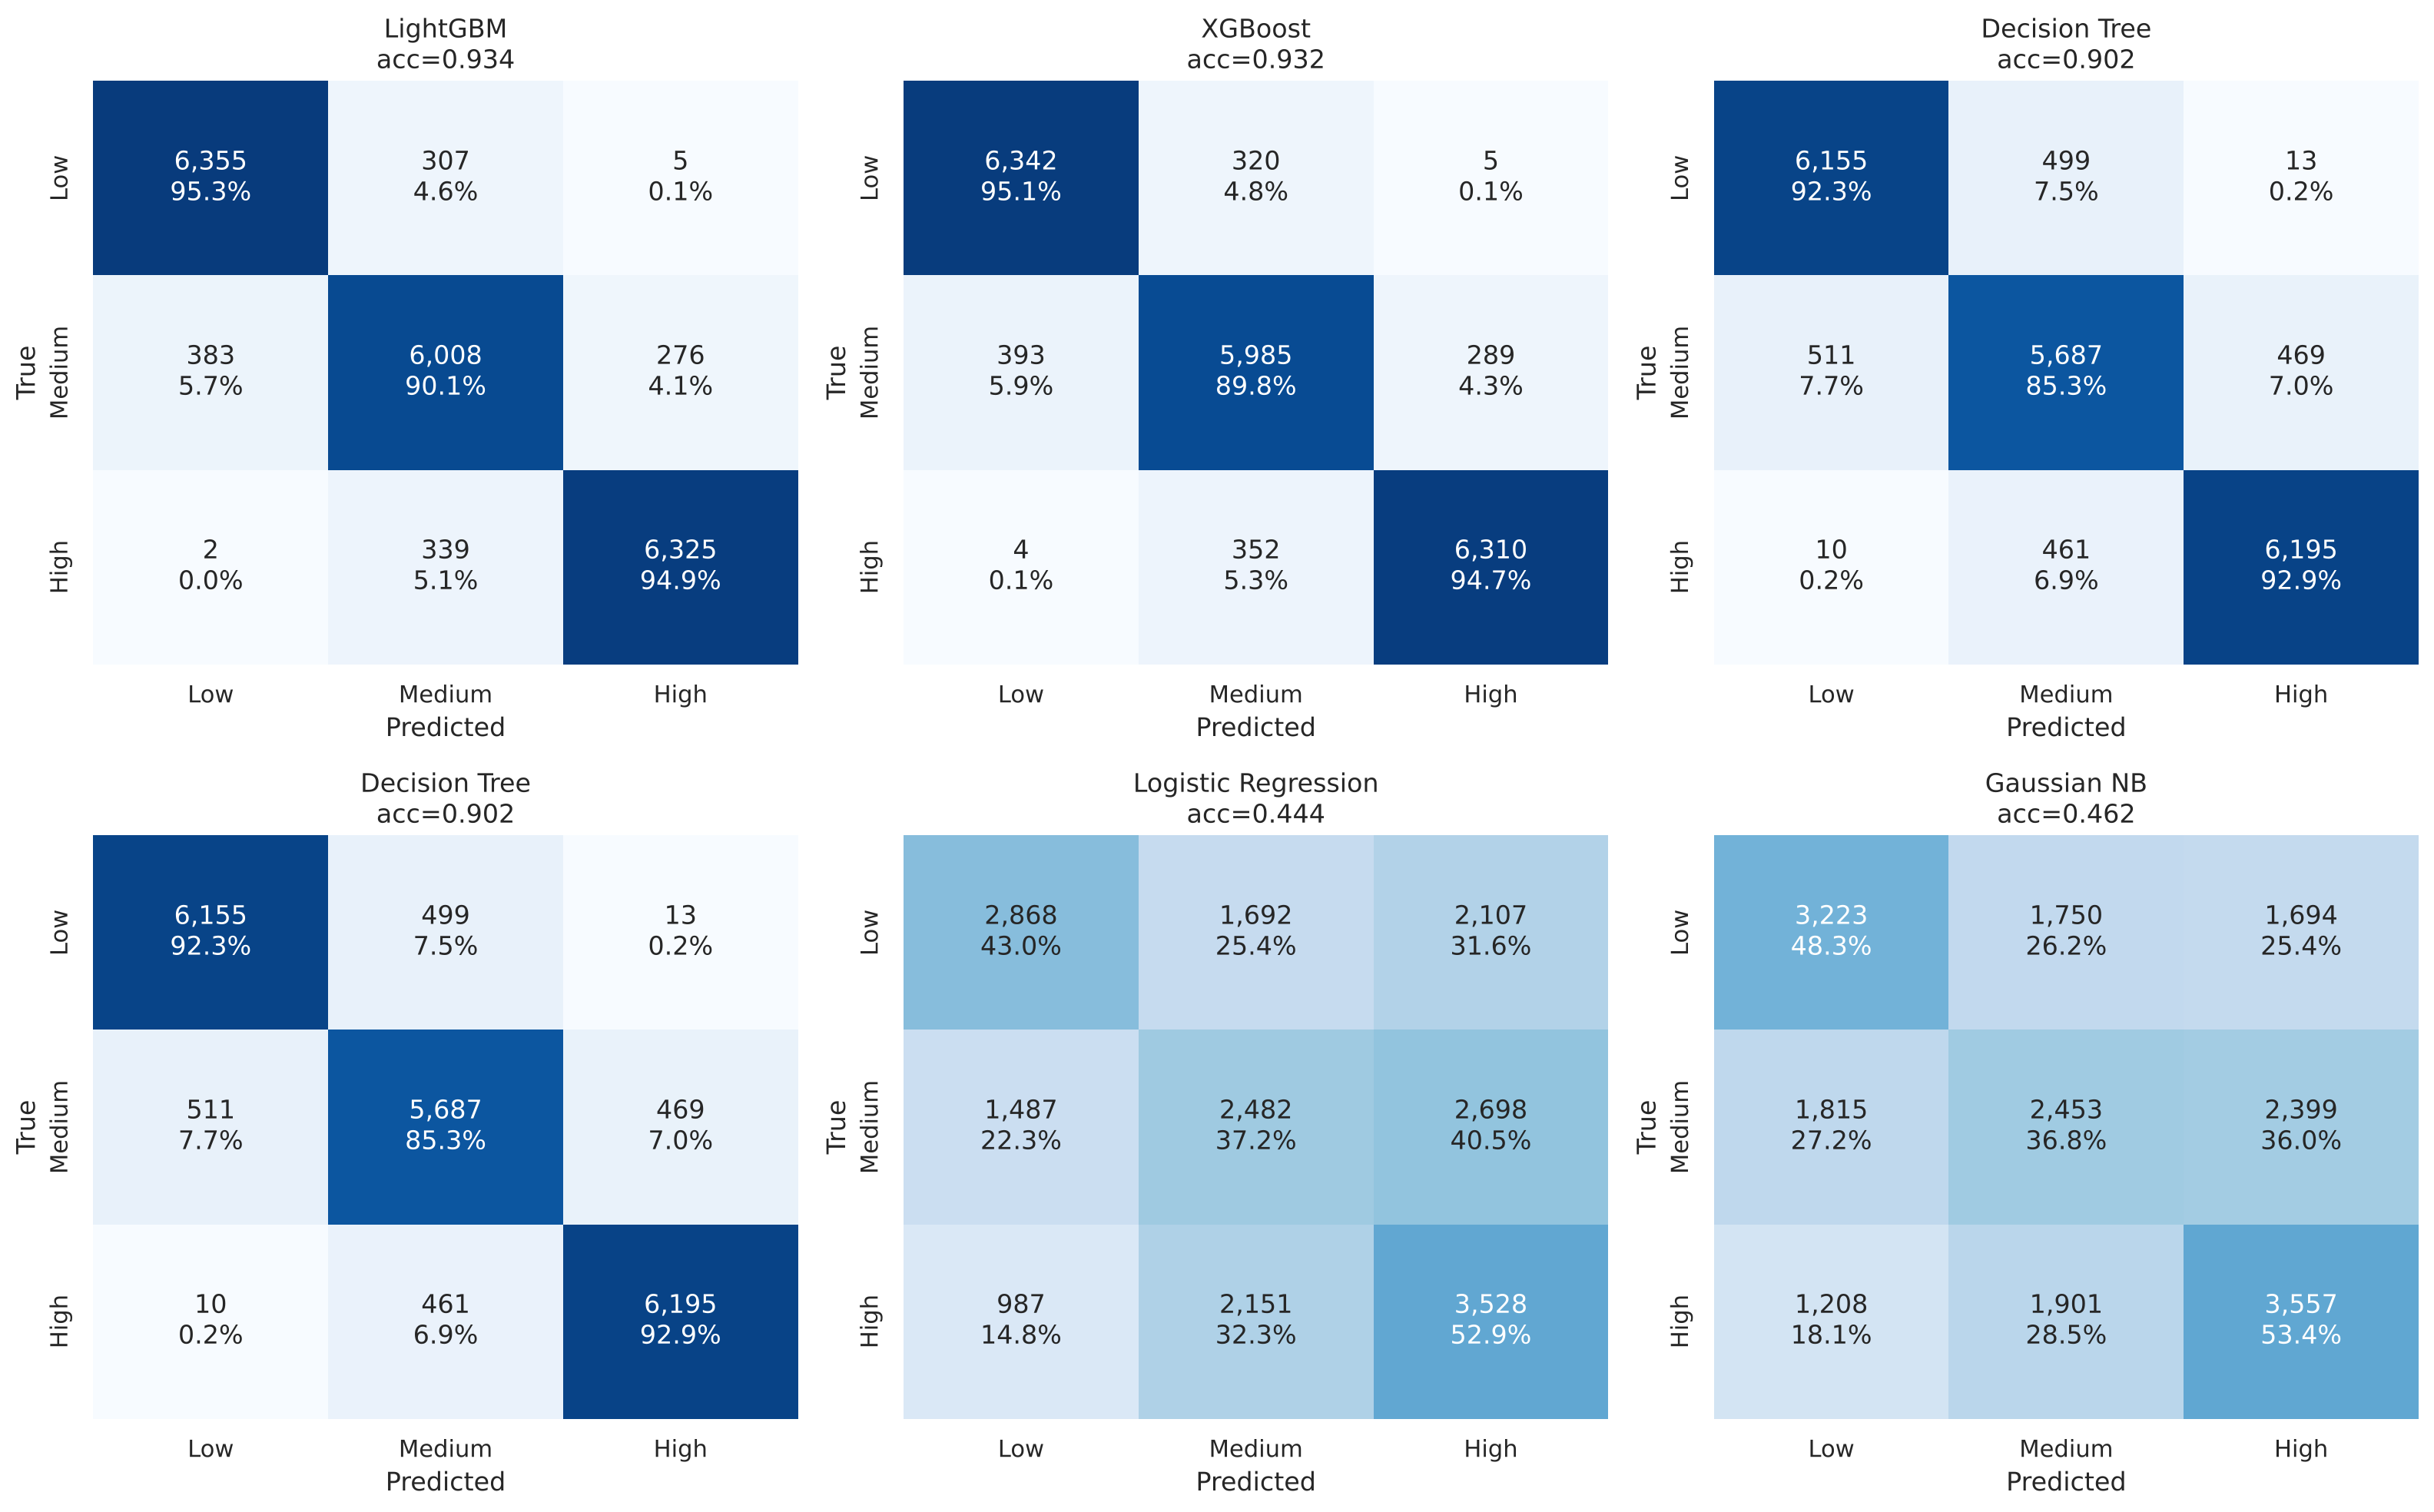
\includegraphics[width=0.9\textwidth]{figures/13_confusion_matrices.png}
\caption{Test-set confusion matrices (counts and row percentages). Top: the three best models. Bottom: the unpruned decision tree and two under-fitting linear/probabilistic models.}
\label{fig:cm}
\end{figure*}

\begin{table}[!t]
\caption{Interpretation of the confusion matrices (test set, 20{,}000 rows)}
\label{tab:cmint}
\centering
\setlength{\tabcolsep}{2.5pt}
\begin{tabular}{lccccc}
\toprule
 & \multicolumn{3}{c}{Recall (L / M / H)} & Errors & Far (L$\leftrightarrow$H) \\
\midrule
LightGBM & 0.953 & 0.901 & 0.949 & 1{,}312 & 7 (0.5\%) \\
XGBoost & 0.951 & 0.898 & 0.947 & 1{,}363 & 9 (0.7\%) \\
Decision Tree & 0.923 & 0.853 & 0.929 & 1{,}963 & 23 (1.2\%) \\
Gaussian NB & 0.483 & 0.368 & 0.534 & 10{,}767 & 2{,}902 (26.9\%) \\
Logistic Reg. & 0.430 & 0.372 & 0.529 & 11{,}122 & 3{,}094 (27.8\%) \\
\bottomrule
\end{tabular}
\end{table}

\subsection{ROC analysis}
Fig.~\ref{fig:roc} shows the one-vs-rest ROC curves of LightGBM (left) and the micro-averaged ROC curves of all nine models (right). The per-class AUCs of LightGBM are 0.995 (Low vs.\ rest), 0.982 (Medium vs.\ rest) and 0.996 (High vs.\ rest). This matches the confusion-matrix finding that the middle class is the hardest to isolate. The ranking of the models by AUC follows their ranking by accuracy, with one notable exception: the random forest and the MLP have modest accuracies (67--69\%) but respectable AUCs (0.850 and 0.852). Their probability \emph{rankings} are therefore much better than their hard decisions, a sign that their errors are concentrated near the decision thresholds.

\begin{figure*}[!t]
\centering
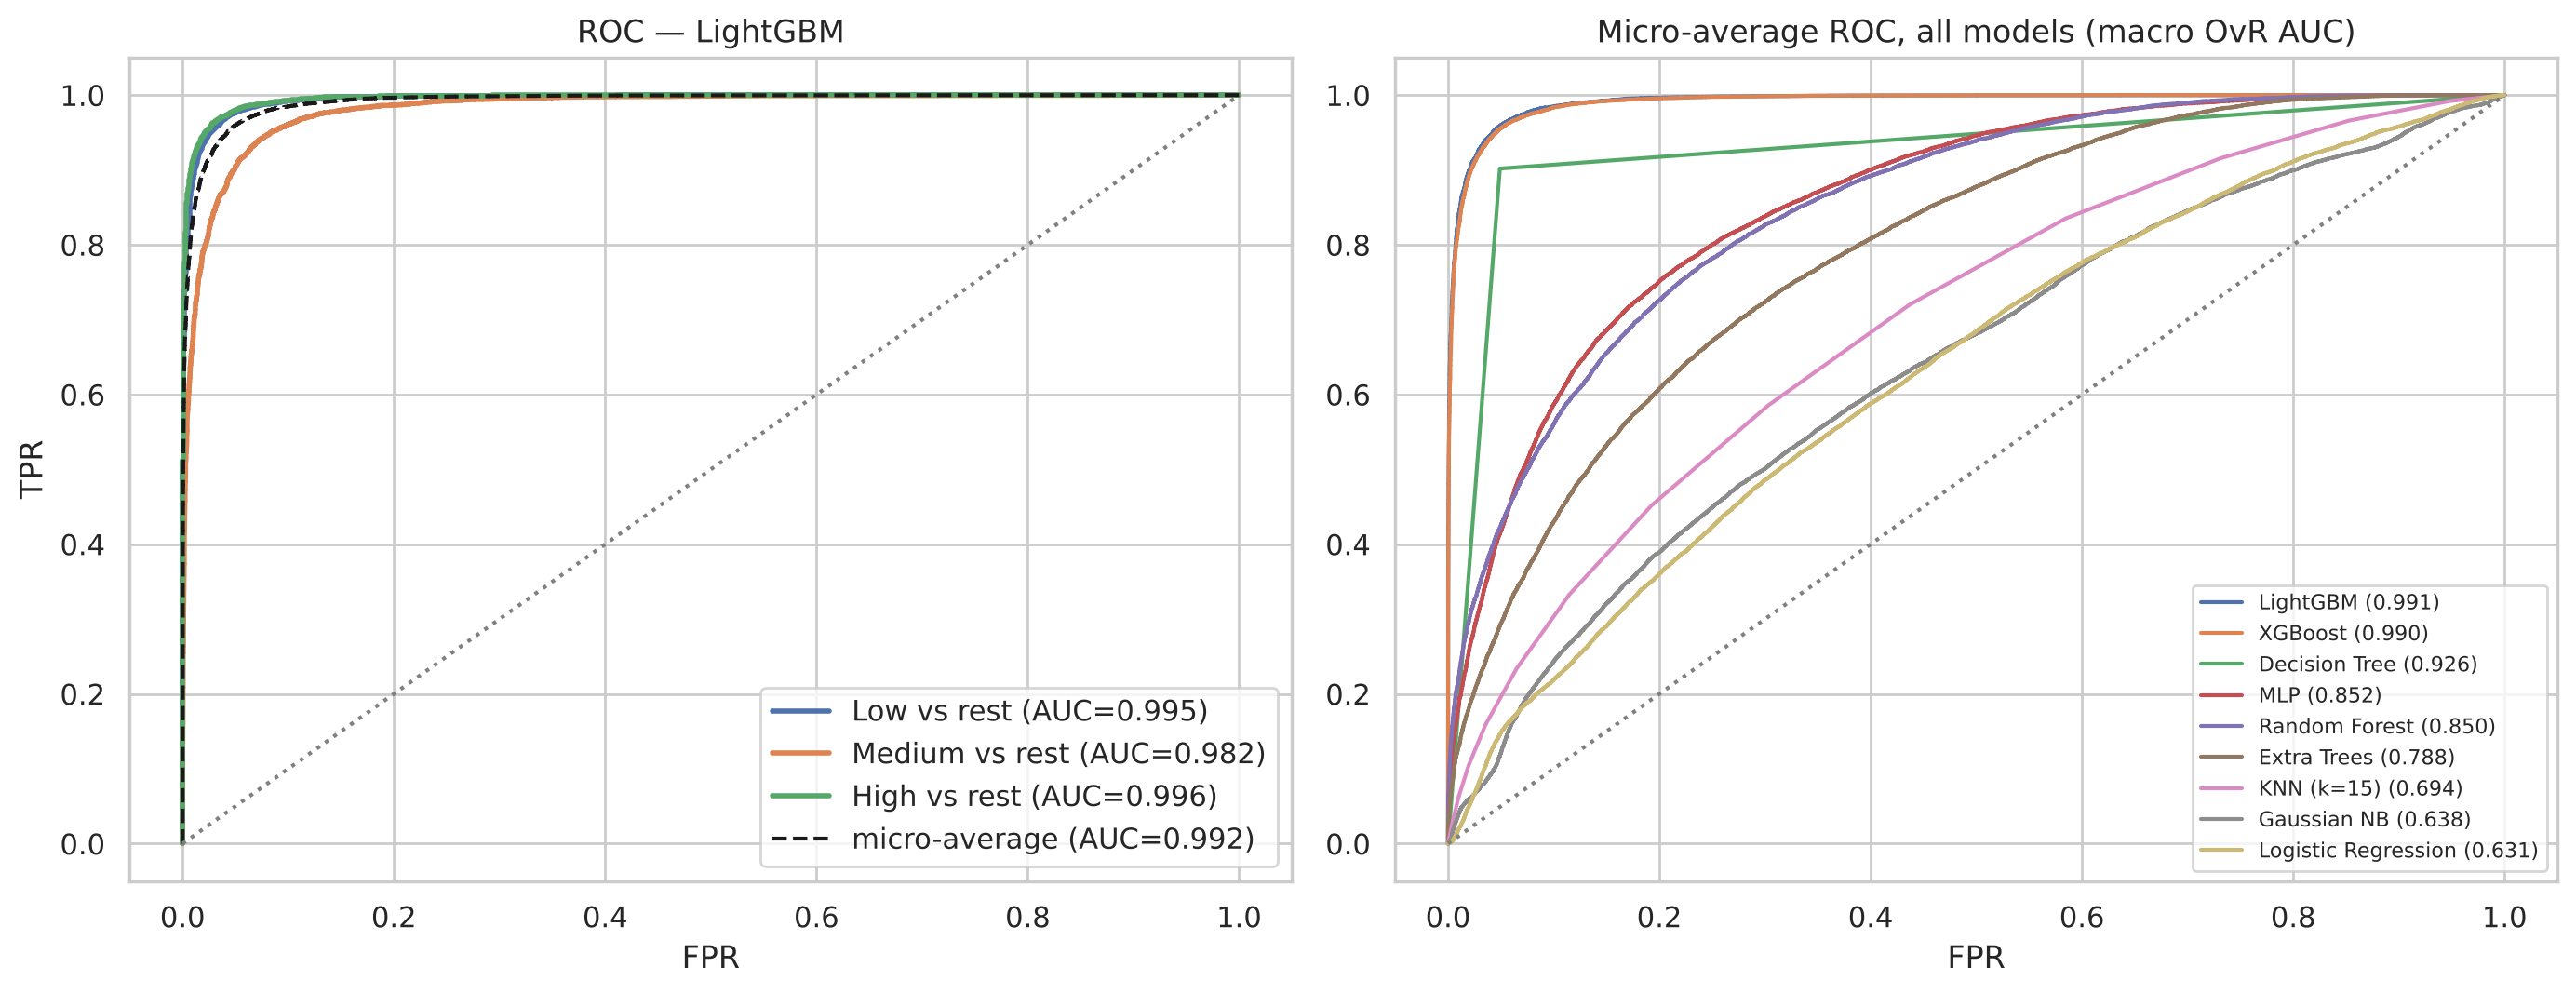
\includegraphics[width=0.9\textwidth]{figures/14_roc_curves.png}
\caption{ROC curves. Left: LightGBM, one-vs-rest per class and micro-average. Right: micro-averaged ROC of all models, with their macro one-vs-rest AUC in the legend.}
\label{fig:roc}
\end{figure*}

\subsection{Over-fitting and under-fitting}
Fig.~\ref{fig:fit} analyses the bias--variance behaviour from three angles.

\emph{Train--test gap} (left panel). Logistic regression and naive Bayes have train and test accuracies that are equal (gaps of $-0.3$ and $-0.6$ points) and both low: pure \textbf{under-fitting} (high bias). The unpruned decision tree is the textbook \textbf{over-fitting} case, with 100\% training accuracy and a 9.8-point gap. The random forest and extra trees show the most severe over-fitting, with gaps of 25.4 and 30.9 points. $k$-NN combines both problems: a low test accuracy (50.8\%) \emph{and} an 8.4-point gap, because with $k=15$ it memorises local neighbourhoods that are dominated by the noisy context variables. LightGBM and XGBoost have moderate gaps (5.9 and 5.6 points) just above our 5-point threshold. Their \emph{test} accuracy is nevertheless the best, so this is benign over-fitting typical of boosted ensembles, not a reason for concern.

\emph{Learning curve of LightGBM} (middle panel). Training accuracy stays at 100\% (99.8\% at full size) while validation accuracy rises steadily from 77.2\% with 2{,}666 rows to 85.5\%, 89.1\%, 91.5\% and 92.6\% with 53{,}333 rows, without plateauing. The remaining gap is therefore a \emph{variance} gap that more data would continue to close: the model has enough capacity, and its limiting factor is the number of examples per store-department combination ($45\times81$ cells with only a few dozen weeks each).

\emph{Validation curve of the decision-tree depth} (right panel). This curve shows the full transition from under- to over-fitting. At depth 2 training and validation accuracies are both 46.9\% (under-fitting). They rise together until depth 8 (76.6\% vs.\ 76.0\%). The validation accuracy peaks at \textbf{depth 16} (89.5\%), and beyond that the training accuracy keeps rising to 100\% while the validation accuracy declines slightly to 89.2\% (over-fitting).

\begin{figure*}[!t]
\centering
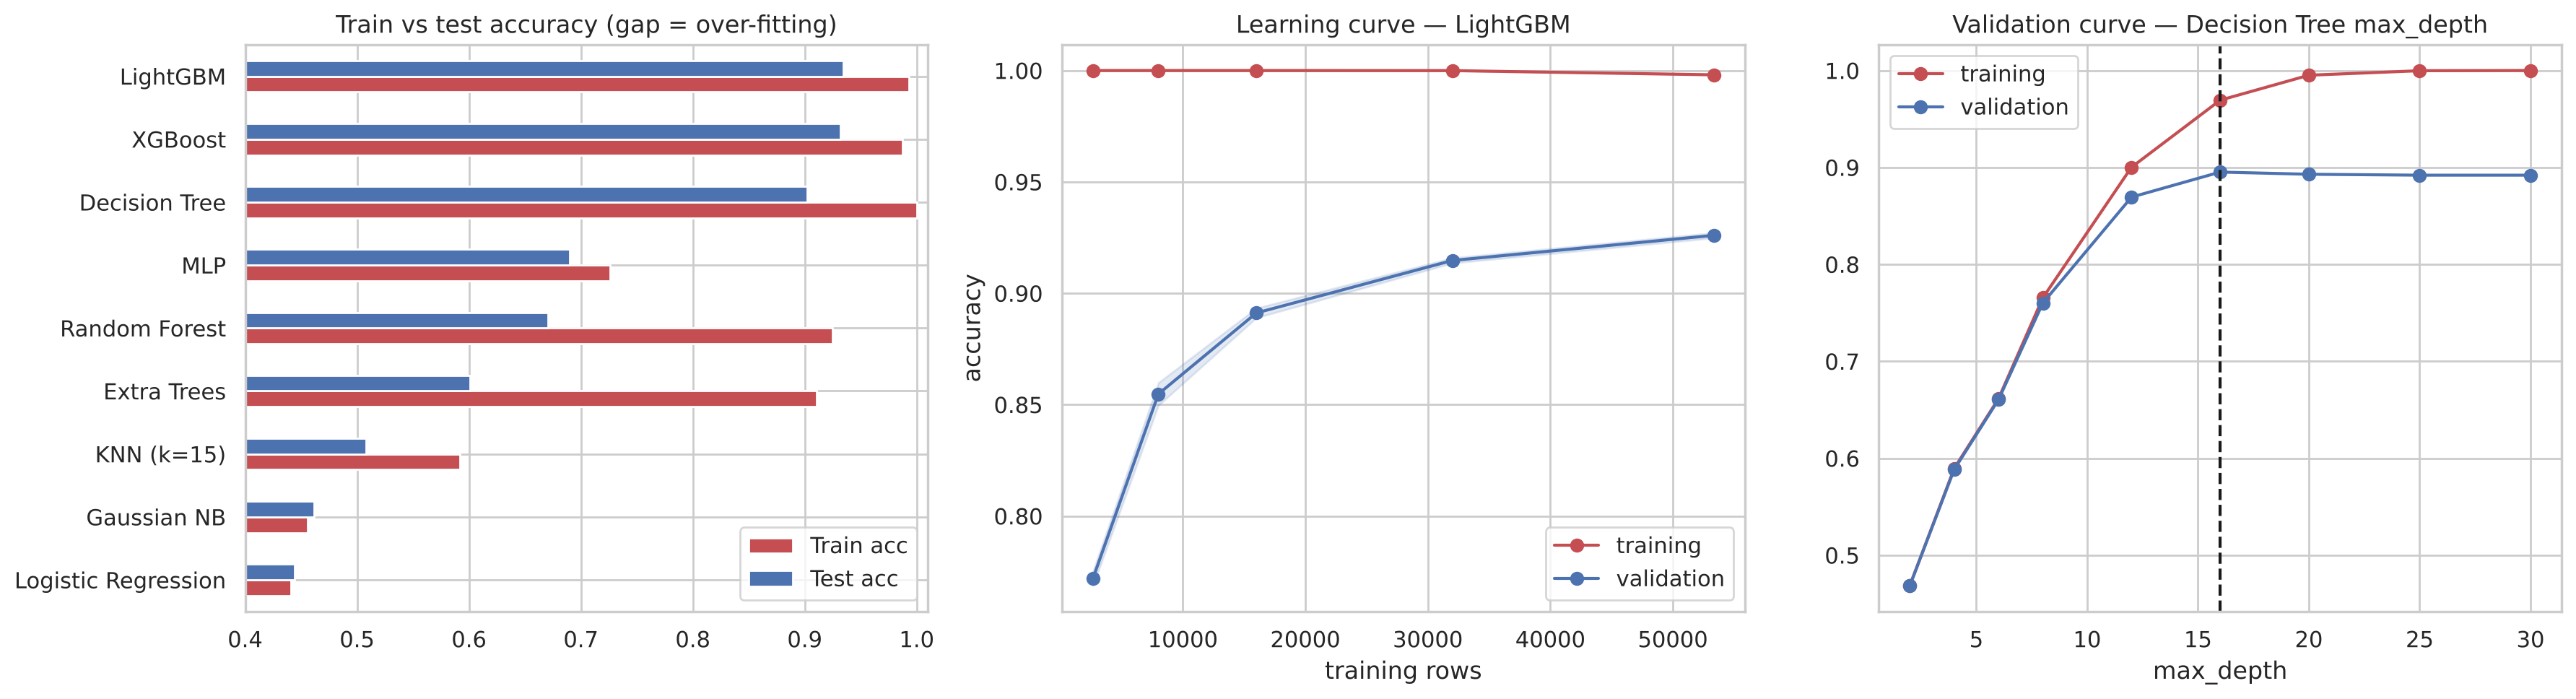
\includegraphics[width=\textwidth]{figures/15_over_under_fitting.png}
\caption{Over-/under-fitting analysis. Left: train vs.\ test accuracy of every model. Middle: learning curve of LightGBM (3-fold, mean $\pm$ std). Right: validation curve of the decision-tree depth, with the optimum at depth 16.}
\label{fig:fit}
\end{figure*}

\subsection{Ablation: why the default forests fail}\label{sec:res:ablation}
The poor results of the random forest (67.1\%) and extra trees (60.1\%) are surprising, given that a single unpruned tree reaches 90.2\%. We hypothesised that the cause is the default \texttt{max\_features}$=\sqrt{d}$. With $d=25$, each split may only consider 5 randomly drawn features, so the dominant \texttt{Dept} variable (67\% of LightGBM's gain) is available at only about 20\% of the splits. The trees are then forced to split on store-week context variables (\texttt{CPI}, \texttt{Temperature}, \texttt{Fuel\_Price}), which are almost unique per store-week and let the trees memorise the training data --- hence the very large train--test gaps.

Table~\ref{tab:ablation} confirms the hypothesis. Raising \texttt{max\_features} to 50\% of the features lifts the random forest from 67.1\% to 91.4\% and extra trees from 60.1\% to 90.5\%. Letting every split see all features (plain bagging) brings them to \textbf{93.0\%} and \textbf{93.3\%}, within 0.2 points of LightGBM, while the train--test gaps shrink from 25--31 points to 3--6 points. The general lesson for mixed-type tabular data is that the random-subspace mechanism, which normally decorrelates trees, becomes harmful when one feature carries most of the signal. The ``failure'' of the default forests is thus a hyper-parameter effect, not a limitation of bagging itself.

\begin{table}[!t]
\caption{Effect of \texttt{max\_features} on the forests (150 trees, minimum leaf 2; same 80/20 split)}
\label{tab:ablation}
\centering
\begin{tabular}{llcccc}
\toprule
Model & max\_feat. & Train & Test & F1 & AUC \\
\midrule
Random Forest & $\sqrt{d}$ (5) & 0.925 & 0.671 & 0.670 & 0.850 \\
 & 0.5 (12) & 0.990 & 0.914 & 0.914 & 0.981 \\
 & 1.0 (25) & 0.989 & \textbf{0.930} & \textbf{0.930} & \textbf{0.988} \\
\midrule
Extra Trees & $\sqrt{d}$ (5) & 0.910 & 0.601 & 0.599 & 0.788 \\
 & 0.5 (12) & 0.998 & 0.905 & 0.905 & 0.977 \\
 & 1.0 (25) & 0.997 & \textbf{0.933} & \textbf{0.933} & \textbf{0.990} \\
\bottomrule
\end{tabular}
\end{table}


\subsection{Effect of reduction and selection on the best model}\label{sec:res:subsets}
Finally, LightGBM was retrained on every selected subset and on three linear projections, using the same 80/20 split (Table~\ref{tab:subsets}, Fig.~\ref{fig:subsets}). Three results stand out.

\begin{enumerate}
\item \textbf{Metaheuristic subsets are the best.} The 6-feature GA subset gives the highest test accuracy of all inputs (\textbf{93.70\%}, F1 0.9369, AUC 0.9915), slightly \emph{above} the full 25-feature model (93.44\%). It does so with 76\% fewer features and 42\% less training time (5.5\,s vs.\ 9.5\,s). BPSO (9 features) is second (93.64\%). SA, with only 5 features, retains 99.8\% of the full model's accuracy (93.22\%). Removing noise variables thus reduces over-fitting as well as cost: the GA model's train--test gap falls to 4.5 points, below the 5-point threshold.
\item \textbf{Non-linear wrappers and embedded selectors are close behind; linear embedded and filter subsets lose accuracy.} RFE (93.54\%), LightGBM-gain (93.46\%) and both SFS variants (93.3--93.4\%) match the full model with 10 features. The L2 subset (91.46\%) and the filter subset (91.04\%) lose 2--2.4 points, because they were chosen by linear or univariate criteria that over-rate the redundant store-type dummies and miss interactions.
\item \textbf{Projections destroy the signal the trees need.} LightGBM on the 16 PCA (or SVD) components drops to 69.7\% accuracy, and on the 2 LDA axes to 51.1\% --- losses of 24 and 42 points. Rotating the data mixes the decisive nominal \texttt{Dept} variable with continuous noise, so the axis-aligned splits that make trees effective are no longer possible. For tree ensembles on mixed-type tabular data, \emph{selection} is clearly preferable to \emph{reduction}.
\end{enumerate}

\begin{table*}[!t]
\caption{LightGBM re-trained on each feature subset or projection (80{,}000 train / 20{,}000 test rows)}
\label{tab:subsets}
\centering
\begin{tabular}{lcccccc}
\toprule
Input & \# dims & Train acc. & Test acc. & Macro-F1 & ROC-AUC & Fit (s) \\
\midrule
GA (metaheuristic) & 6 & 0.9823 & \textbf{0.9370} & \textbf{0.9369} & \textbf{0.9915} & 5.5 \\
BPSO (metaheuristic) & 9 & 0.9826 & 0.9364 & 0.9364 & 0.9915 & 5.7 \\
RFE (wrapper) & 10 & 0.9922 & 0.9354 & 0.9354 & 0.9910 & 6.2 \\
LightGBM gain (embedded) & 10 & 0.9907 & 0.9346 & 0.9346 & 0.9911 & 6.6 \\
All features & 25 & 0.9929 & 0.9344 & 0.9344 & 0.9906 & 9.5 \\
SFS backward (wrapper) & 10 & 0.9864 & 0.9342 & 0.9342 & 0.9909 & 7.2 \\
SFS forward (wrapper) & 10 & 0.9695 & 0.9332 & 0.9332 & 0.9907 & 5.1 \\
Elastic-Net (embedded) & 21 & 0.9921 & 0.9330 & 0.9330 & 0.9903 & 8.4 \\
SA (metaheuristic) & 5 & 0.9695 & 0.9322 & 0.9322 & 0.9907 & 5.0 \\
L1 / Lasso (embedded) & 19 & 0.9920 & 0.9322 & 0.9322 & 0.9903 & 8.4 \\
L2 / Ridge (embedded) & 10 & 0.9569 & 0.9146 & 0.9146 & 0.9859 & 5.3 \\
Filter, rank fusion & 10 & 0.9622 & 0.9104 & 0.9103 & 0.9841 & 6.2 \\
PCA, 16 comp.\ (95\% var.) & 16 & 0.9017 & 0.6968 & 0.6960 & 0.8761 & 9.5 \\
SVD, 16 comp. & 16 & 0.9017 & 0.6968 & 0.6960 & 0.8761 & 9.9 \\
LDA, 2 axes & 2 & 0.6018 & 0.5108 & 0.5104 & 0.6984 & 4.5 \\
\bottomrule
\end{tabular}
\end{table*}


\begin{figure}[!t]
\centering
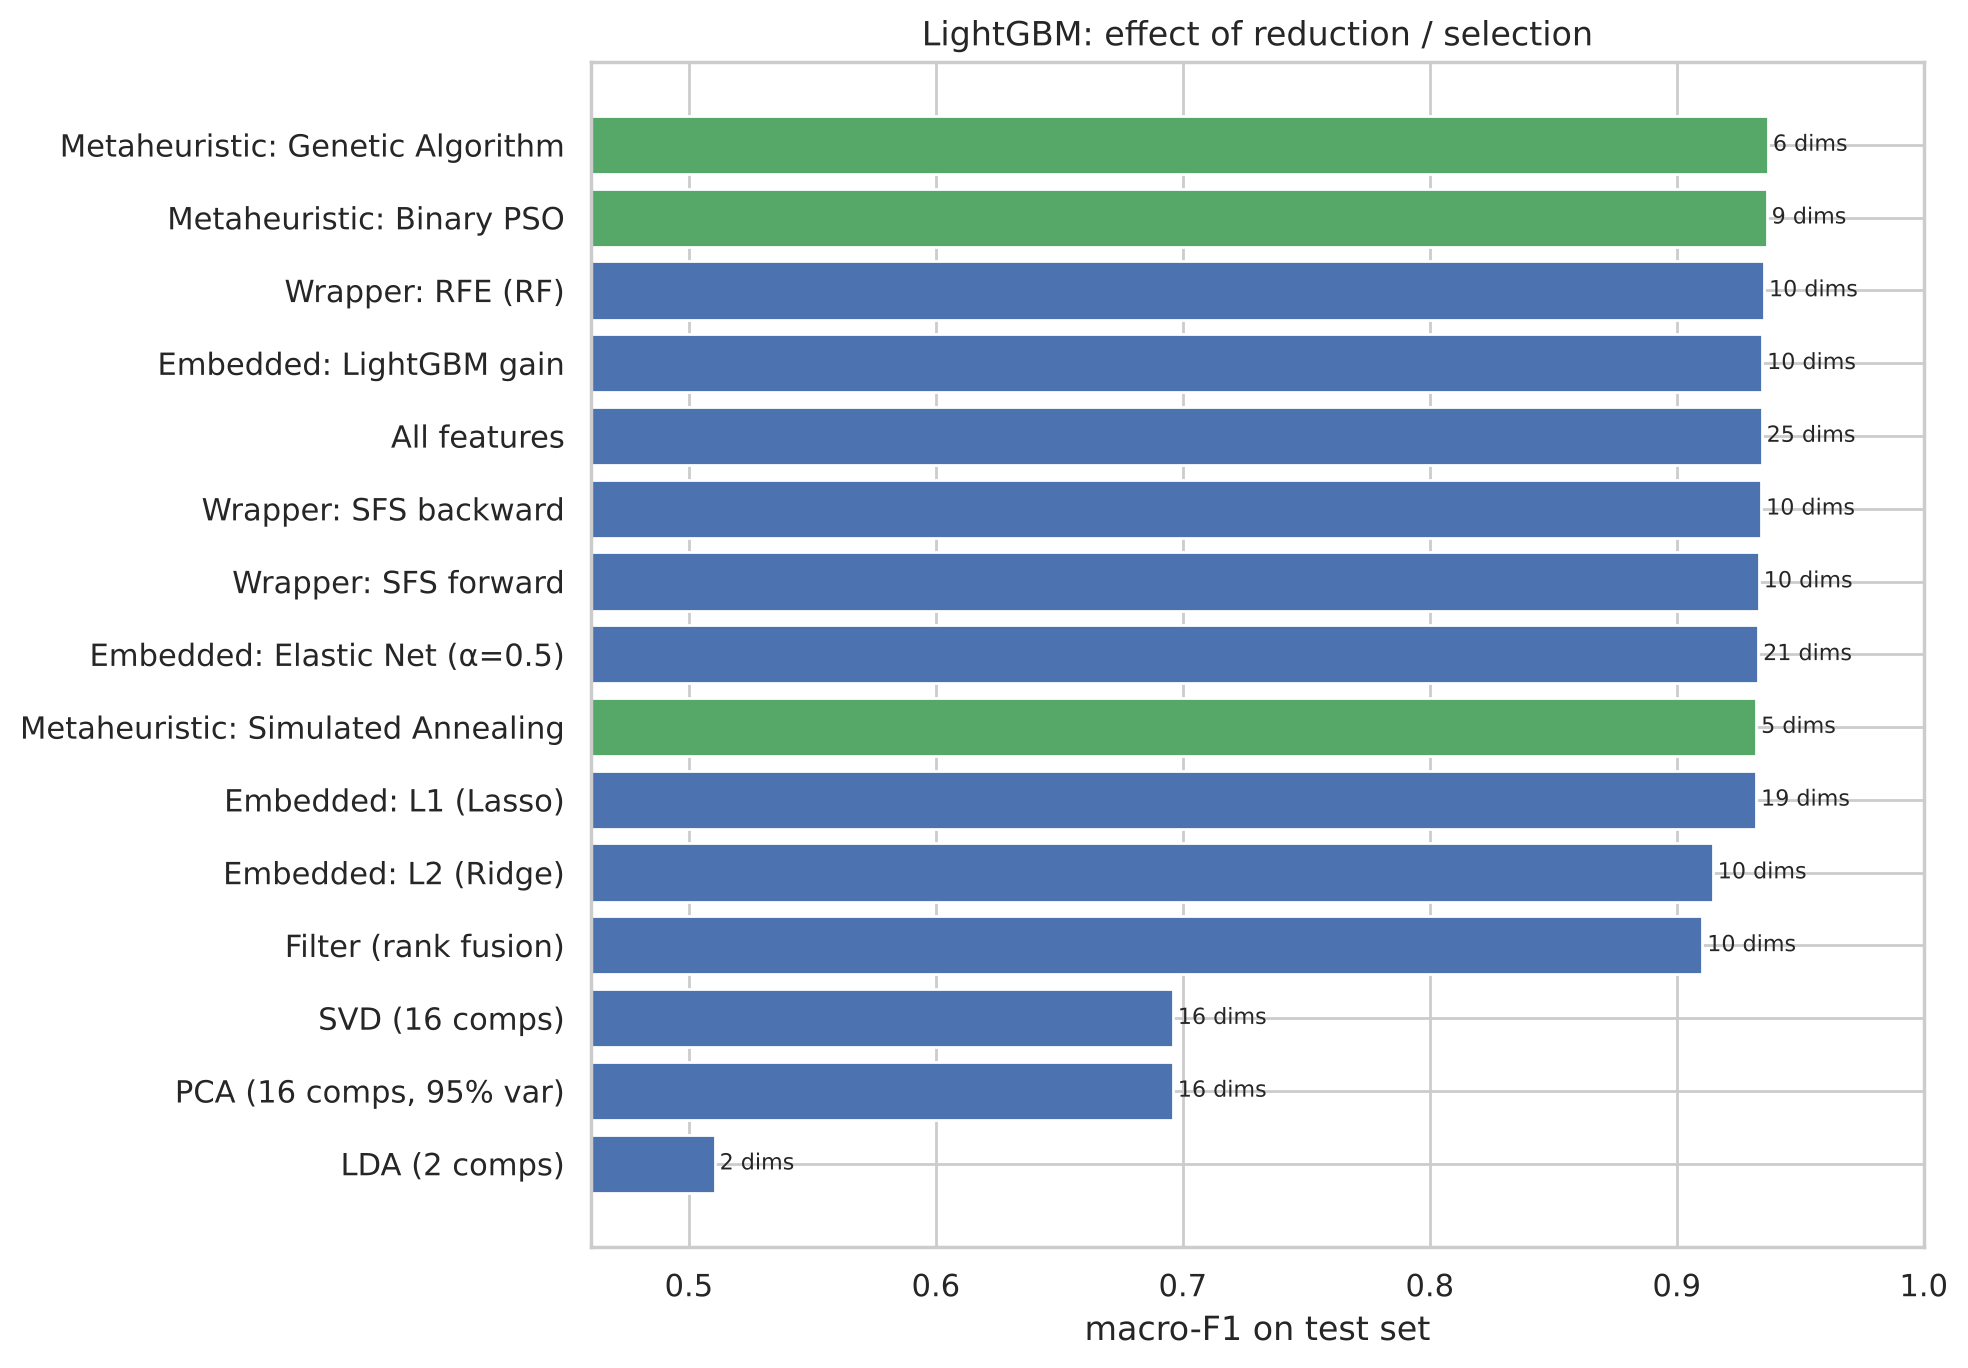
\includegraphics[width=\columnwidth]{figures/16_subset_comparison.png}
\caption{Test macro-F1 of LightGBM for every feature subset and projection (number of input dimensions annotated). Metaheuristic subsets are shown in green.}
\label{fig:subsets}
\end{figure}

%========================================================================
\section{Comparison with Related Work}\label{sec:compare}
%========================================================================
Table~\ref{tab:related} positions this study against published work on the same Walmart data. A direct numeric comparison is not possible: all previous studies predict the sales \emph{amount} (regression) and report $R^2$, MAE, RMSE or SMAPE, while we predict the sales \emph{level} (classification) and report accuracy, F1 and AUC. Moreover, Chen~\cite{chen2022} and Punati \emph{et al.}~\cite{punati2025} use the aggregated store-level version of the data (one row per store-week), whose errors are measured in hundreds of thousands of dollars, whereas we work at the far noisier department level. The comparison is therefore one of \emph{approach} and \emph{findings}, and on these terms the studies agree with ours in four respects:

\begin{itemize}
\item \textbf{Boosted trees are the strongest conventional learners.} Chenwi \emph{et al.}~\cite{chenwi2024} and Akande \emph{et al.}~\cite{akande2022} found XGBoost to be the best regressor, and only the much more complex Temporal Fusion Transformer of~\cite{punati2025} beat it. In our classification setting LightGBM and XGBoost are likewise the top two models by a large margin.
\item \textbf{Linear models are inadequate at the department level.} Chen~\cite{chen2022} obtained a reasonable fit with linear regression on \emph{store-level} aggregates, where the department identity has been summed out. At the department level our linear and naive-Bayes classifiers under-fit badly (44--46\%), for the same structural reason.
\item \textbf{Over-fitting is the main risk of flexible models.} The polynomial model of~\cite{chen2022} reached a high training $R^2$ but an exploding test RMSE; in our study the unpruned tree and the default forests show the same pattern, and the validation curve locates the optimum tree depth.
\item \textbf{Store identity, department and size dominate.} Chen~\cite{chen2022} identified type and size as the most influential variables, and our eleven selectors unanimously confirm \texttt{Store}, \texttt{Dept} and \texttt{Size}, while finding the economic and promotional variables of secondary importance.
\end{itemize}

What this study adds is the systematic treatment of the feature space, which none of the cited works attempts. We compare ten reduction techniques with quantitative quality criteria, show that unsupervised clustering does not recover sales segments, compare four families of feature selection including three metaheuristics, and demonstrate that a 6-feature GA subset matches or exceeds the full model while selection before reduction improves embeddings by more than ten points.

\begin{table*}[!t]
\caption{Comparison with related work on the Walmart sales data. Regression and classification metrics are not directly comparable}
\label{tab:related}
\centering
\begin{tabular}{p{2.6cm}p{2.6cm}p{3.4cm}p{3.1cm}p{4.2cm}}
\toprule
Study & Task / granularity & Models & Feature reduction / selection & Best reported result \\
\midrule
Chen (2022)~\cite{chen2022} & Regression, store level & MLR, Elastic-Net, polynomial & None (manual) & MLR $R^2=0.933$; ENR $R^2=0.814$; polynomial over-fits \\
Akande et al.\ (2022)~\cite{akande2022} & Regression & XGBoost & Not reported & XGBoost judged effective \\
Yao (2023)~\cite{yao2023} & Regression, dept.\ level & DT, RF, KNN regressors & None & RF $R^2=0.937$, MAE $=1937.8$ \\
Chenwi et al.\ (2024)~\cite{chenwi2024} & Regression & LR, RF, GBM, XGBoost, LightGBM & None & XGBoost MAE $=1226.5$, $R^2\approx0.9999$ \\
Punati et al.\ (2025)~\cite{punati2025} & Multi-horizon forecasting, store level & XGB, CNN, LSTM, CNN-LSTM, TFT & None & TFT $R^2=0.9875$, SMAPE $4.51\%$ \\
\midrule
\textbf{This work} & \textbf{3-class sales level, dept.\ level} & 9 classifiers; 10 reduction methods; K-Means & Filter, wrapper (SFS, RFE), embedded (L1, L2, EN, gain), GA, BPSO, SA & LightGBM: acc.\ 93.44\%, F1 0.934, AUC 0.991; GA (6 feat.): acc.\ 93.70\%, AUC 0.992 \\
\bottomrule
\end{tabular}
\end{table*}

%========================================================================
\section{Discussion}\label{sec:discussion}
%========================================================================
\subsection{Why the problem is hard for some models and easy for others}
The results can be explained by one structural fact: the sales level of a department-week is determined mainly by \emph{which} department of \emph{which} store it is, and these are nominal identifiers coded as integers. A tree can isolate an arbitrary set of department numbers with a few splits; a linear model, a Gaussian naive Bayes or a distance-based $k$-NN cannot, because for them department 92 is simply ``more'' than department 91. The same fact explains why unsupervised embeddings and K-Means fail to show the classes: distances are dominated by the 20 context variables that vary from week to week, while the decisive information sits in a single identifier dimension. It also explains why selection helps reduction (Section~\ref{sec:res:ras}) and why PCA and LDA projections hurt the trees (Section~\ref{sec:res:subsets}).

\subsection{The value of metaheuristic selection}
The GA, BPSO and SA did not merely match the deterministic selectors; they produced the smallest subsets with the best test performance. The size penalty in Eq.~(\ref{eq:fitness}) is essential here. Greedy wrappers were run with a fixed target size ($K=10$) and filled the remaining slots with weakly useful variables, whereas the metaheuristics discovered that five or six features suffice. The three algorithms reached almost the same core subset, which supports the robustness of the result, although no single metaheuristic dominates on every problem~\cite{wolpert1997}. Their cost, a few minutes each, was made acceptable by three design choices: a 20k-row selection sample, a fast 60-tree surrogate learner and fitness caching.

\subsection{Limitations and threats to validity}
\begin{itemize}
\item \textbf{Random rather than temporal split.} We split rows randomly, as the project specification requires. Because each store-department appears in both training and test weeks, the classifier partly memorises its typical level. A forward-chaining time split would be the right protocol for a deployed forecaster and would give lower scores.
\item \textbf{Sampling.} Computing limits led us to use a 100k-row stratified sample for modelling, 20k rows for selection and 1k--3k points for manifold learning. The learning curve suggests that LightGBM would gain about one more percentage point from the full data.
\item \textbf{Tertile thresholds.} The class boundaries are statistical, not business-defined. Most errors occur close to them, so a different cut (for example store-specific thresholds) would change the absolute numbers but probably not the ranking.
\item \textbf{Hyper-parameters.} The classifiers use sensible defaults rather than a full search. The forest ablation shows that a single hyper-parameter can change the ranking of a model family, and a nested search (possibly itself metaheuristic) is a natural next step.
\item \textbf{Stochasticity.} Each metaheuristic was run with one seed. Repeated runs would quantify their variance more precisely.
\end{itemize}

%========================================================================
\section{Conclusion and Future Work}\label{sec:conclusion}
%========================================================================
We re-formulated Walmart department-level sales prediction as a balanced three-class sales-level problem and used it to compare feature-reduction, feature-selection and classification methods on a large, noisy, mixed-type dataset. Six findings stand out:

\begin{enumerate}
\item LightGBM is the best classifier: 93.44\% hold-out accuracy, macro-F1 0.934 and ROC-AUC 0.991, confirmed by 5-fold CV (93.42\% $\pm$ 0.20\%). Its errors are almost all between adjacent levels; only 0.5\% are Low$\leftrightarrow$High.
\item Linear, probabilistic and distance-based classifiers under-fit (44--51\%) because \texttt{Dept} is a nominal identifier. Default random forests and extra trees over-fit and under-perform a single tree; the ablation attributes this to \texttt{max\_features} hiding the dominant variable.
\item Among ten 2-D embeddings, t-SNE and UMAP preserve neighbourhoods best (trustworthiness $\ge$0.99) and supervised LDA preserves class information best (46.3\% kNN accuracy). No unsupervised embedding or K-Means clustering recovers the sales levels, even when its silhouette is high.
\item Feature selection before reduction raises the class information in PCA, t-SNE and UMAP embeddings by 11--13 points.
\item All eleven selectors agree that \texttt{Store}, \texttt{Dept} and \texttt{Size} are essential. The GA finds a 6-feature subset that slightly exceeds the 25-feature model (93.70\% accuracy) with 42\% less training time, and BPSO and SA find comparable 9- and 5-feature subsets.
\item For tree ensembles on tabular data, feature \emph{selection} preserves accuracy while linear \emph{projection} (PCA, LDA) destroys it.
\end{enumerate}

Future work will (i) evaluate the pipeline with a forward-chaining temporal split, (ii) replace integer identifiers by target or embedding encodings so that linear and distance-based methods (and unsupervised reduction) can use them, (iii) jointly optimise feature subsets and hyper-parameters with a multi-objective metaheuristic such as NSGA-II, trading accuracy against subset size and training time, and (iv) extend the classification view to cost-sensitive and ordinal formulations that penalise Low$\leftrightarrow$High errors more heavily.


\section*{Reproducibility}
All experiments are contained in the notebook \texttt{Modeling.ipynb} (Phase~1 section). The notebook re-creates every table and figure of this paper from the raw Kaggle files with a fixed random seed (42), and stores all reported numbers in \texttt{results/phase1\_results.json}.

\bibliographystyle{IEEEtran}
\bibliography{refs}

\end{document}
